\documentclass[14pt,usenames,dvipsnames,professionalfonts]{beamer}


% =======================================================================
% Packages & definitions
% =======================================================================
\usepackage[orientation=portrait,size=a3,scale=1.0,debug]{beamerposter}
%\usepackage[orientation=portrait,a0,scale=1.0,debug]{beamerposter}

% =======================================================================
%% Font packages (see http://www.ctan.org/topic/font-greek)
% =======================================================================
% \usepackage[english,greek]{babel} 
% \usepackage[utf8]{inputenc}
% %\usepackage{lmodern}     %ruins some characters (for example, \Delta in math mode)
% \usepackage{kmath,kerkis} %use kmath for better math letters!
% \usepackage[T1]{fontenc}

%\usepackage{fontspec}
%\setsansfont{Liberation Serif}
%\usepackage[english]{babel} 
%\usepackage[utf8]{inputenc}
%\usepackage{lmodern}
%\usepackage{kmath}
%\usepackage[T1]{fontenc}
\usepackage[T1]{fontenc}
% =======================================================================
%% Other packages
% =======================================================================
\usepackage[ddmmyyyy, dayofweek, 24hr]{datetime} % usage: \longdate
\usepackage{tabularx}
\usepackage{float}
\usepackage[countmax]{subfloat}
%\usepackage{showkeys} %uncomment to use. modifies the \label,\ref,\pageref, \cite and \bibitem commands so that the `internal' key is printed.
\usepackage{fancybox}
\usepackage{subfig}
% \let\subfigure\subfloat% compatibility between subfigure and subfig packages 
\usepackage{ifthen}
\usepackage{xcolor}
\usepackage{xspace} 
\usepackage{textcomp} %for degrees symbol 
\usepackage{epsfig}
\usepackage{graphicx}
\usepackage{amsmath,amssymb}% for advanced math typesetting % amsmath provides split
\usepackage{fancyhdr} %enables use of heaters/footers
\usepackage{bibentry} % for in-line full citations
\usepackage{gensymb} %for degrees symbol
\usepackage{tcolorbox}
\usepackage{multicol}
\usepackage{multimedia} % can be used to show movies (mp4, avi, etc..) with: \movie[options]{}{film.avi}
\usepackage{kantlipsum} 
\usepackage{nicefrac}
\usepackage{eso-pic} %position logo anywhere you want
\usepackage{textcomp,mathcomp} % degrees celcius
\usepackage[weather]{ifsym} % sun symbol
\usepackage{lipsum}
\usepackage{dirtytalk}
\usepackage{wrapfig}

% =======================================================================
%% TikZ packages
% =======================================================================
\usepackage{varwidth}
\usepackage{tikz}
%\usepackage{animate}
\usepackage{media9}
\usetikzlibrary{decorations.pathmorphing}
\usetikzlibrary{decorations.markings}
\usetikzlibrary{decorations.pathreplacing}
 \usetikzlibrary{decorations.text}
\usetikzlibrary{shapes}
\usetikzlibrary{patterns}
\tcbuselibrary{skins, xparse}
\usetikzlibrary{calc}
\tcbuselibrary{hooks}
%\usepackage{pgfplots,tikz}
\usetikzlibrary{automata,positioning}
\usetikzlibrary{arrows.meta}


% =======================================================================
%% Setup Hyperref package: Enables hyper-referencing 
% =======================================================================
\usepackage{hyperref}
\hypersetup{
  plainpages=false, 
  unicode=true,                      % non-Latin (e.g. Greek) characters in Acrobat bookmarks?
  pdftoolbar=false,                  % show Acrobat toolbar?
  pdfmenubar=false,                  % show Acrobat menu?
  pdffitwindow=false,                % window fit to page when opened?
  pdfstartview={FitV},               % fits the page-width to the window?
  pdftitle={Fotios Ptochos},         % title of the document
  pdfsubject={Particle Physics},     % subject of the document
  pdfcreator={Alexandros Attikis},   % creator of the document
  pdfauthor={Alexandros Attikis},    % author of the document
  pdfproducer={Beamer/LaTeX},        % producer of the document
  pdfkeywords={{Fotios}{Ptochos}{Professor}{UCY}{Physics}{HEP}{CMS}{CERN}{FNAL}}, %keywords?
  pdfnewwindow=false,                % links in new window?
  colorlinks=false,                  % false: boxed links ,  true: colored links
  linkcolor=black,                   % color of internal links
  citecolor=black,                   % color of links to bibliography
  filecolor=black,                   % color of file links
  urlcolor=black,                    % color of external links
}

%\newcommand{\en}{\selectlanguage{english}}
%\newcommand{\gr}{\selectlanguage{greek}}

\newcommand\PutLogo[3]{%
  \AtPageLowerLeft{%
    \put(\LenToUnit{#1\paperwidth},\LenToUnit{#2\paperheight}){#3}}%
}

\newcommand{\MakePosterLogos}[4]{ %%% do NOT remove '%' at line end`
  \AddToShipoutPictureFG{
    \PutLogo{0.010}{0.924}{\includegraphics[height=0.10\paperwidth,keepaspectratio]{./figures/logos/#1}}%
    \PutLogo{0.115}{0.924}{\includegraphics[height=0.10\paperwidth,keepaspectratio]{./figures/logos/#2}}%
    \PutLogo{0.785}{0.924}{\includegraphics[height=0.10\paperwidth,keepaspectratio]{./figures/logos/#3}}%
    \PutLogo{0.890}{0.924}{\includegraphics[height=0.10\paperwidth,keepaspectratio]{./figures/logos/#4}}%
%    \PutLogo{0.1}{0.925}{\includegraphics[width=0.10\paperwidth,keepaspectratio]{./figures/logos/#1}}%
%    \PutLogo{0.0}{0.925}{\includegraphics[width=0.10\paperwidth,keepaspectratio]{./figures/logos/#2}}%
%    \PutLogo{0.8}{0.925}{\includegraphics[width=0.10\paperwidth,keepaspectratio]{./figures/logos/#3}}%
%    \PutLogo{0.9}{0.925}{\includegraphics[width=0.10\paperwidth,keepaspectratio]{./figures/logos/#4}}%
  }
}

\newcommand{\MakePosterColumns}[3]{
\newlength{\ColumnWidth}
\setlength{\ColumnWidth}{0.315\paperwidth}
\begin{columns}[t]
    \begin{columns}[t,totalwidth=1.0\paperwidth] % split up that three-column-wide column
      \begin{column}{\ColumnWidth} \input{./tex/#1.tex} \end{column}
      \begin{column}{\ColumnWidth} \input{./tex/#2.tex} \end{column}
      \begin{column}{\ColumnWidth} \input{./tex/#3.tex} \end{column}    
    \end{columns}
  \end{columns}
}

% =======================================================================
% Colour definitions. See: http://en.wikipedia.org/wiki/Web_colors
% =======================================================================
%\definecolor{kOldPaper}   {RGB}{250, 252, 243}
%\definecolor{kOldPaperAlt}{RGB}{254, 241, 226}
\definecolor{kOldPaper}   {RGB}{231, 229, 220}
\definecolor{kOldPaperV1} {RGB}{250, 252, 243}
\definecolor{kBlack}      {RGB}{  0,   0,   0}
\definecolor{kWhite}      {RGB}{255, 255, 255}
\definecolor{kPink}       {RGB}{227,  74, 147}
\definecolor{kNavyBlue}   {RGB}{ 28, 130, 185}
\definecolor{kDarkBlue}   {RGB}{  0,   0, 214}
\definecolor{kLightBlue}  {RGB}{  0,  61, 245}
\definecolor{kvLightBlue} {RGB}{  0, 184, 245}
\definecolor{kMyBlue}     {RGB}{ 51, 102, 255}
\definecolor{kHLTausBlue} {RGB}{ 11,  36, 251}
\definecolor{kBlue}   {RGB}{ 51, 102, 255}
\definecolor{kGreen}  {RGB}{ 98, 158,  31}
\definecolor{kLightGreen}{RGB}{223, 254,  191}
\definecolor{kRed}    {RGB}{220,   0,   0}
\definecolor{kOrange} {RGB}{230, 120,  20}
\definecolor{kYellow} {RGB}{255, 221,   0}
\definecolor{kBlue}   {RGB}{ 10,  50, 150}
\definecolor{kBrown}  {RGB}{120,  89,  30}
\definecolor{kPink}   {RGB}{255,   0, 128}

% =======================================================================
% Customise tcolorboxes (package "tcolorbox")
% =======================================================================
\tcbset{
    noparskip,
    coltitle  = green,
    colframe  = pink,
    colback   = orange,
    coltext   = yellow,
    fonttitle =\normalsize, 
    posterStyle/.style = {coltitle=red, colframe=brown, colback=brown, coltext=red, fonttitle = \Large},
    boxsep       = +0.20cm,   % Title Box Height
    top          = +0.50cm,   % Top Margin (from Title box line)
    bottom       = +0.00cm,   % Bottom Margin 
    left         = +0.10cm,   % Left Margin
    right        = +0.10cm,   % Right Margin
    toptitle     = +0.10cm,   % ?
    bottomtitle  = +0.10cm,   % ?
    arc          = +0.8cm,
    nobeforeafter,
    %center title,
}
    
% new tcolorbox environment
\newtcolorbox{headline}[2][]{
  coltext          = black,
  colframe         = black, %gray!50
  colback          = \MyBlockFillColorRight,
  colbacktitle     = \MyBlockTitleBoxColor,
  coltitle         = black,
  title            = #2,
  fonttitle        = \bfseries\Huge,
  boxrule          = 0pt, % border line width
  % opacityframe     = 0,   % remove box border line
  titlerule       = 1pt,
  % colbacktitle    = red!50!yellow,
  % titlerule style = black,
  titlerule style = {black, arrows = {Hooks [arc=270]-Hooks [arc=270]}},
  opacityback     = 1.0, % 1.0 means totally transparent, 0.0 means totally opaque
  top             =-0.0cm,
  bottom          = 0.0cm,
  left            = 0.05cm,
  right           = 0.05cm,
  arc             = 0.0cm, % 0.0cm for non-rounded corners!
  sharp corners,
  frame hidden,
  parbox=false,
  #1,
}

% new tcolorbox environment
\newtcolorbox{SubArticle}[2][]{
  coltext      = black,
  colframe     = black, %gray!50
  colback      = \MyBlockFillColorRight,
  colbacktitle = \MyBlockTitleBoxColor,
  coltitle     = black,
  title        = #2,
  fonttitle    = \bfseries\large,
  boxrule      = 0pt, % border line width
  % opacityframe = 0,   % remove box border line
  titlerule    = 1pt,
  % colbacktitle    = red!50!yellow,
  % titlerule style = black,
  %titlerule style = {black, arrows = {Hooks [arc=270]-Hooks [arc=270]}},
  opacityback     = 1.0, % 1.0 means totally transparent, 0.0 means totally opaque
  top             = +0.00cm,
  bottom          = +0.00cm,
  left            = +0.05cm,
  right           = +0.05cm,
  arc             = +0.00cm, % 0.0cm for non-rounded corners!
  sharp corners,
  frame hidden,
  parbox=false,
  #1,
}

% new tcolorbox environment
\newtcolorbox{MyArticle}[2][]{
  coltext      = black,
  colframe     = black, %gray!50, %\MyBlockFrameColorLeft,
  colback      = \MyBlockFillColorRight, %white, %\MyBlockFillColorLeft,
  colbacktitle = \MyBlockTitleBoxColor,
  coltitle     = black,
  title        = {\Large{\textbf{#2}}},
  fonttitle    = \bfseries,
  boxrule      = 0pt, %frame line width
  % borderline   = {1mm}{0mm}{solid}, % dashed  {dot width}{margin width}
  titlerule    = 0pt, %tiitle line width
  opacityback  = 1.0, % 1.0 means totally transparent, 0.0 means totally opaque
  top          = -0.20cm,
  bottom       = +0.00cm,
  left         = +0.05cm,
  right        = +0.05cm,
  arc          = +0.00cm, % 0.0cm for non-rounded corners!
  sharp corners,
  #1,
}

% new tcolorbox environment
\newtcolorbox{MyArticleDotted}[2][]{
  coltext      = black,
  colframe     = black, %gray!50, %\MyBlockFrameColorLeft,
  colback      = \MyBlockFillColorRight, %white, %\MyBlockFillColorLeft,
  colbacktitle = \MyBlockTitleBoxColor,
  coltitle     = black,
  title        = {\Large{\textbf{#2}}},
  fonttitle    = \bfseries,
  boxrule      = 0pt, %frame line width
  borderline={1mm}{0mm}{dotted}, % dashed  {dot width}{margin width}
  titlerule    = 0pt, %tiitle line width
  %tikz={rotate=#3}, % manipulate the tcolorbox as a whole (in degrees)
  top=-0.0cm, bottom=+0.0cm, left=+0.05cm, right=+0.05cm,
  %enlarge top by   = +1.0cm,  %  equivalent to mdframed 'skipabove'
  %enlarge bottom by= +0.0cm,  %  equivalent to mdframed 'skipbelow'
  %enlarge left by  = +1.5cm,  
  %enlarge right by = +0.0cm, 
  opacityback=1.0, % 1.0 means totally transparent, 0.0 means totally opaque
  arc=0.0cm,        % 0.0cm for non-rounded corners!
  sharp corners,
  #1,
}

% new tcolorbox environment
\newtcolorbox{MyArticleDashed}[2][]{
  coltext      = black,
  colframe     = black, %gray!50, %\MyBlockFrameColorLeft,
  colback      = \MyBlockFillColorRight, %white, %\MyBlockFillColorLeft,
  colbacktitle = \MyBlockTitleBoxColor,
  coltitle     = black,
  title        = {\Large{\textbf{#2}}},
  fonttitle    = \bfseries,
  boxrule      = 0pt, %frame line width
  borderline={1mm}{0mm}{dashed}, % dashed  {dot width}{margin width}
  titlerule    = 0pt, %tiitle line width
  %tikz={rotate=#3}, % manipulate the tcolorbox as a whole (in degrees)
  top=-0.0cm, bottom=+0.0cm, left=+0.05cm, right=+0.05cm,
  %enlarge top by   = +1.0cm,  %  equivalent to mdframed 'skipabove'
  %enlarge bottom by= +0.0cm,  %  equivalent to mdframed 'skipbelow'
  %enlarge left by  = +1.5cm,  
  %enlarge right by = +0.0cm, 
  opacityback=1.0, % 1.0 means totally transparent, 0.0 means totally opaque
  arc=0.0cm,        % 0.0cm for non-rounded corners!
  sharp corners,
  #1,
}


\newtcolorbox{multimuons-1}[2][]{ 
  coltext      = black,
  colframe     = black, %\MyBlockFrameColorLeft,
  colback      = \MyBlockFillColorRight, %white, %\MyBlockFillColorLeft,
  colbacktitle = \MyBlockTitleBoxColor,
  coltitle     = black,
  title        = {\Large{\textbf{#2}}},
  fonttitle    = \bfseries,
  boxrule      = 0pt, %frame line width
  titlerule    = 0pt, %tiitle line width
  titlerule style = {white},
  %tikz={rotate=#3}, % manipulate the tcolorbox as a whole (in degrees)
  top=-0.0cm, bottom=+0.0cm, left=+0.05cm, right=+0.05cm,
  %enlarge top by   = +1.0cm,  %  equivalent to mdframed 'skipabove'
  %enlarge bottom by= +0.0cm,  %  equivalent to mdframed 'skipbelow'
  %enlarge left by  = +1.5cm,  
  %enlarge right by = +0.0cm, 
  opacityback=1.0, % 1.0 means totally transparent, 0.0 means totally opaque
  arc=0.0cm,        % 0.0cm for non-rounded corners!
  sharp corners,
  frame hidden,
  #1,
}

\newtcolorbox{multimuons-2}[2][]{ 
  coltext      = black,
  colframe     = black, %\MyBlockFrameColorLeft,
  colback      = \MyBlockFillColorRight, %white, %\MyBlockFillColorLeft,
  colbacktitle = \MyBlockTitleBoxColor,
  coltitle     = black,
  title        = {\Large{\textbf{#2}}},
  fonttitle    = \bfseries,
  boxrule      = 1pt, %frame line width
  titlerule    = 0pt, %tiitle line width
  titlerule style = {white},
  %tikz={rotate=#3}, % manipulate the tcolorbox as a whole (in degrees)
  top=-0.2cm, bottom=+0.0cm, left=+0.05cm, right=+0.05cm,
  %enlarge top by   = +1.0cm,  %  equivalent to mdframed 'skipabove'
  %enlarge bottom by= +0.0cm,  %  equivalent to mdframed 'skipbelow'
  %enlarge left by  = +1.5cm,  
  %enlarge right by = +0.0cm, 
  opacityback=1.0, % 1.0 means totally transparent, 0.0 means totally opaque
  arc=0.0cm,        % 0.0cm for non-rounded corners!
  sharp corners,
  frame hidden,
  #1,
}




\newtcolorbox{MyColumnLeft}[3][]{
  coltext      = \MyFontColor,
  colframe     = \MyBlockFrameColorLeft,
  colback      = \MyBlockFillColorLeft,
  colbacktitle = \MyBlockTitleBoxColor,
  coltitle     = \MyHeadingsColor,
  title        = \Large{\bfseries{#2\\}},
  boxrule      = 0.2cm, %frame line width
  height       = #3,
  enlarge top by   = +1.0cm,  %  equivalent to mdframed 'skipabove'
  enlarge bottom by= +0.0cm,  %  equivalent to mdframed 'skipbelow'
  enlarge left by  = +1.5cm,  
  enlarge right by = +0.0cm, 
  #1,
}

\newtcolorbox{MyColumnCenter}[3][]{
  coltext      = \MyFontColor,
  colframe     = \MyBlockFrameColorCenter,
  colback      = \MyBlockFillColorCenter,
  colbacktitle = \MyBlockTitleBoxColor,
  coltitle     = \MyHeadingsColor,
  title        = \Large{\textbf{#2\\}},
  boxrule      = 0.2cm, %frame line width
  height       = #3,
  enlarge top by   = +1.0cm,  %  equivalent to mdframed 'skipabove'
  enlarge bottom by= +0.0cm,  %  equivalent to mdframed 'skipbelow'
  enlarge left by  = +0.0cm,  
  enlarge right by = +0.0cm, 
   #1,
}


% new tcolorbox environment
\newtcolorbox{MyColumnRight}[3][]{
  coltext      = \MyFontColor,
  colframe     = \MyBlockFrameColorRight,
  colback      = \MyBlockFillColorRight,
  colbacktitle = \MyBlockTitleBoxColor,
  coltitle     = \MyHeadingsColor,
  title        = \Large{\textbf{#2\\}},
  boxrule      = 0.2cm, %frame line width
  height       = #3,
  enlarge top by   = +1.0cm,  %  equivalent to mdframed 'skipabove'
  enlarge bottom by= +0.0cm,  %  equivalent to mdframed 'skipbelow'
  enlarge left by  = -1.5cm,
  enlarge right by = +0.0cm,
  #1,
}

% =======================================================================
% Block format/colour definitions
% =======================================================================
\newcommand{\CustomiseColours}[9]{
  \newcommand{\MyFontColor}{#1}
  \newcommand{\MyHeadingsColor}{#2}
  \newcommand{\MyBlockFillColorLeft}{#3}
  \newcommand{\MyBlockFrameColorLeft}{#3}
  \newcommand{\MyBlockFillColorCenter}{#4}
  \newcommand{\MyBlockFrameColorCenter}{#4}
  \newcommand{\MyBlockFillColorRight}{#5}
  \newcommand{\MyBlockFrameColorRight}{#5}
  \newcommand{\MyBlockTitleBoxColor}{#6}
  \newcommand{\MyBackgroundColour}{#7}
  \newcommand{\MyFooterFontColour}{#8}
  \newcommand{\MyFooterFillColour}{#9}
  \setbeamercolor{background canvas}{bg=\MyBackgroundColour}
  \setbeamertemplate{navigation symbols}{}
  \setbeamercolor{block title}{fg=\MyFontColor, bg=black}
  \setbeamercolor{block body} {fg=\MyBlockFillColor, bg=black} 
  \setbeamercolor{block alerted title}{fg=red, bg=pink}
  \setbeamercolor{block alerted body} {fg=red, bg=pink}
  \setbeamercolor{title in head/foot}{fg=\MyFooterFontColour, bg=\MyFooterFillColour}
}

% =======================================================================
% Footer
% =======================================================================
\setbeamercolor{title in head/foot}{fg=black, bg=\MyBackgroundColour}
\newcommand{\FooterHeight}{0.8cm}
\newcommand{\FooterBoxDepth}{0.6cm} % The depth of a box is the distance between the baseline and the bottom of the box;

% Footer
\newcommand{\SetFooterText}[1]{
  \setbeamertemplate{footline}{
    \leavevmode
    \hbox{\begin{beamercolorbox}[wd=1.0\paperwidth,ht=\FooterHeight, dp=\FooterBoxDepth, leftskip=0.01\paperwidth, rightskip=0.01\paperwidth]{title in head/foot}
        \usebeamerfont{title in head/foot}  \centering \normalsize{#1}
      \end{beamercolorbox}
    }
  }
}

% Footer (Alternative)
\newcommand{\CustomiseFooterAlt}[3]{
  \setbeamercolor{title in head/foot}{fg=#1,bg=#2}
  \setbeamertemplate{footline}{
    \leavevmode
    \hbox{\begin{beamercolorbox}[wd=1.0\paperwidth, ht=\FooterHeight, dp=\FooterBoxDepth]{title in head/foot}
        \usebeamerfont{title in head/foot}  \centering \normalsize{#3}
      \end{beamercolorbox}
    }
  }
}


% =======================================================================
% Figures
% =======================================================================
\newcommand{\oneSubFig}[3]{
  \includegraphics[width=#3\textwidth,keepaspectratio]{figures/#2}
  \label{fig:#1}
}

\newcommand{\oneFigPosterNoCaption}[3]{
  \begin{figure}[tbp]  
      \begin{columns}
        \begin{column}{0.99\textwidth}
          \centering
          \includegraphics[width=#3\textwidth,keepaspectratio]{figures/#2}
          \label{fig:#1}
        \end{column}
      \end{columns}
  \end{figure}
}


\newcommand{\oneFigPoster}[4]{
  \begin{figure}[tbp]
    \def\figurename{Εικόνα}
      \begin{columns}
        \begin{column}{0.99\textwidth}
          \centering
          \includegraphics[width=#3\textwidth,keepaspectratio]{figures/#2}
          \label{fig:#1}
        \end{column}
      \end{columns}
    \caption{#4}
  \end{figure}
}

\newcommand{\twoFigPoster}[6]{
  \begin{figure}[tbp]
    \def\figurename{Εικόνα}
      \begin{columns}
        \begin{column}{0.47\textwidth}
          \oneSubFig{#1_a}{#2}{#3}
        \end{column}
        \begin{column}{0.47\textwidth}
          \oneSubFig{#1_b}{#4}{#5}
        \end{column}
      \end{columns}
    \caption{#6}
  \end{figure}
}

\newcommand{\twoFigPosterNoCaption}[5]{
  \begin{figure}[tbp]
      \begin{columns}
        \begin{column}{0.47\textwidth}
          \oneSubFig{#1_a}{#2}{#3}
        \end{column}
        \begin{column}{0.47\textwidth}
          \oneSubFig{#1_b}{#4}{#5}
        \end{column}
      \end{columns}
  \end{figure}
}

\newcommand{\twoFigColumnsPoster}[6]{
  \begin{figure}[tbp]
    \begin{columns}
      \begin{column}{0.5\textwidth}
        \begin{tcolorbox}[posterStyle]
          \oneSubFig{#1_a}{#2}{#3}
    \end{tcolorbox}
      \end{column}
      \begin{column}{0.5\textwidth}
        \begin{tcolorbox}[posterStyle]
          \oneSubFig{#1_b}{#4}{#5}
    \end{tcolorbox}       
      \end{column}
  \end{columns}
    \caption{#6}
  \end{figure}
}

% =======================================================================
% Enumerate Customisations (TikZ)
% =======================================================================
\newcommand*\circled[2]{\tikz[baseline=(char.base)]{  \node[circle, ball color=#2, inner sep=0.1cm] (char) {\textcolor{kWhite}#1};}}
\newcommand*\rounded[2]{\tikz[baseline=(char.base)]{ \node[draw=none,ball color=#2, shade, rounded corners=3.5pt, inner sep=0.1cm] (char) {\textcolor{kWhite}{#1}};}}

\input{./tex/LatexCommands.tex}


% =======================================================================
% Define column width and poster size
% =======================================================================
\usetheme{confposter}


% =======================================================================
% Define Colours
% =======================================================================
\CustomiseColours
    {red!50!white} % \MyFontTitleColor
    {red!30!black} % \MyHeadingsColor
    {kOldPaper}    % \MyBlockFillColorLeft (fill color of main body in tcolorboxes)
    {kOldPaper}    % \MyBlockFillColorCente (?)
    {kOldPaper}    % \MyBlockFillColorRight
    {kOldPaper}    % \MyBlockTitleBoxColor (fill color of heading section in tcoloorboxes)
    {kOldPaper}    % \MyBackgroundColour (entire poster background colour. tcolorbooxes are independent)
    {black}        % \MyFooterTextColour
    {kOldPaper}    % \MyFooterFillColour
    
% =======================================================================
% Define Footer
% =======================================================================
%\SetFooterText{some ads go here. Actual or fake vintange MPEMPA/Tocayo etc.. apple watch? iphone }%
% \CustomiseFooterAlt{kBlack}{kWhite}{
% \rule{\paperwidth}{0.5mm}
% \begin{multicols*}{2}
%     
% \begin{flushleft}
%   EXCITEMENT IN HIGH ENERGY PHYSICS 
% \end{flushleft}
% \columnbreak
% \begin{flushright}
%   AN ASSOCIATE PROFESSOR IS GONE. A PROFESSOR HAS COME
% \end{flushright}
% \end{multicols*}
% }
    

% =======================================================================
% Title block (logos, title, authors, institutes)
% =======================================================================
%\PutLogo{0.010}{0.924}{\includegraphics[height=0.10\paperwidth,keepaspectratio]{./figures/NewspaperTitle.png}}
%\MakePosterLogos{logo_mc}{logo_eu}{logo_cms}{NewspaperTitle}
%\title{The 2022 Chronicle}
\author{Fotios Ptochos\inst{1}}
\institute{\inst{1}{University of Cyprus, Nicosia, Cyprus}}
%\date{\longdate\formatdate{17}{11}{2022}} %\today
\def\MyDate{\longdate\formatdate{17}{11}{2022}} %\today

\setbeamersize
{
    text margin left=0.2cm,
    text margin right=0.2cm
}

% =======================================================================
% Begin document
% =======================================================================
\begin{document}

%\MakePosterColumns{ColumnOne}{ColumnTwo}{ColumnThree}
%\input{./tex/Contents_v1.tex}
%\input{./tex/Contents_v2.tex}
%\input{./tex/Contents_v3.tex}
%\input{./tex/Contents_Alt.tex} % C. Leonidou changes
%\input{./tex/Contents_v4.tex}  % with multicols* (too symmetric. second multicols* changes page!)
%\input{./tex/Contents_v5.tex}
\begin{columns}[T]
  \begin{column}{0.66\textwidth}
    %\begin{headline}[enhanced, tikz={rotate=0}]{Fotios Ptochos Promoted to Professor!}
\begin{headline}[enhanced, tikz={rotate=0}, width=1.0\textwidth]{Fotios Ptochos Promoted to Professor!}
\begin{multicols}{2}
    Congratulations to Fotios Ptochos for his promotion to the rank of
    Full Professor, effective from \MyDate. This promotion recognizes
    Prof. Ptochos' achievements in scholarship, teaching in physics
    and research in high-energy physics (HEP), and his overall service
    to the CDF and CMS Collaborations. He is a Harvard University PhD
    in physics graduate (1998) and has been active in HEP-research%,
    %both in detector development and physics analyses since 1987.
    since 1987. In particular, from 1987 to 1988 he worked in the development of
    a technique to monitor the purity of Liquid Argon (LAr) for the
    first ever prototype of the ICARUS detector.
    %, a technique that was subsequently used in the experiment. 
    From 1989 to 1994 he worked in the characterization of
    various Tetramethyl liquids as part of a research project to find
    appropriate warm liquids media for the envisioned calorimeter
    detectors at the Superconducting Supercollider (SSC).He also
    worked in the construction, installation and 
    calibration of the Central Muon Extension (CMX) system for the CDF
    detector. From 1994 to 1996 he developed an algorithm to improve
    electron identification for the CDF end-plug ECAL based on the
    information from the calorimeter and hits on the silicon tracker
    detector. The algorithm led to the development and implementation of
    the PHOENIX tracker system in the CDF-II detector. 
    %
    In the period of 2000–2003, he was the coordinator of the group
    responsible for the development, installation, maintenance and
    performance monitoring of the CDF-II Hadronic Calorimeter (HCAL)
    timing system. For the entire period of the Tevatron Run-II
    (2001-2011) he served as the coordinator of the CDF central HCAL
    calibration (CHA and WHA), maintenance and performance group. Since
    2004, when he joined the faculty of the UCY Physics Department, he has
    been involved in the UCY HEP group activities related to the
    construction and running of the CMS ECAL at CERN. In 2009, he
    initiated the involvement of the group in the activities related to
    the CMS tracking detector. He was also involved in the development of
    the dual-readout calorimetry concept in a total absorption HCAL for
    future linear-collider experiments. 
    % ========================
    \begin{figure}
      \begin{center}
      \leavevmode
      \includegraphics[width=0.45\textwidth]{./figures/Fotis7.png}
      \end{center}
    \end{figure}
    % ========================
    %
    % ========================
%    \begin{wrapfigure}{l}{0.33\textwidth}
%      \begin{center}
%        \includegraphics[width=0.22\textwidth]{./figures/Fotis7.png}
%      \end{center}
%      %\caption*{Fotios}
%    \end{wrapfigure}
    % ========================
    Professor Ptochos has led numerous physics analyses, spanning
    from precision measurements on properties of heavy flavour quark
    production and their use as probes for searching for the SM and SUSY
    Higgs bosons, to searches for BSM physics including SUSY, extra
    dimensions and other exotic processes. He has tremendous experience in
    heavy flavour tagging techniques and algorithms, tau-lepton
    identification techniques and new physics model building. 
    He was the first ever recipient of the \say{Fermi National
      Accelerator Laboratory Fellowship} and has co-coordinated multiple research program
    funded primarily by the European Commission (EC) via \textsc{Marie
    Skłodowska-Curie Actions},  the Cyprus Research Promotion
    Foundation (RPF) through \textsc{Didaktor} or \textsc{Excellence
      Hubs} programs, the European Regional Development Fund, and
    UCY. Professor Ptochos is the author and co-author of more than 
    1850 publications in refereed scientific journals and a member of the
    editorial group in charge for producing the education material
    for the entire Cyprus Secondary Education. He has been the
    supervisor of the research activities of 6 postdoctoral fellows, 5
    PhD and 11 MSc students, as well as projects of more than 20
    undergraduate students.  
\end{multicols}
\end{headline}


  \end{column}
  \begin{column}{0.33\textwidth}
    \begin{MyArticle}[enhanced, tikz={rotate=0}]{\huge Top Quark, Last Piece of Matter, Appears to Be in Place}
  \begin{multicols}{2}
    We establish the existence of the top quark using a 67 pb$^{-1}$ data
    sample of pp collisions at $\sqrt{s} = 1.8$ TeV collected with the Collider
    Detector at Fermilab (CDF). Employing techniques similar to those we
    previously published, we observe a signal consistent with $t\bar{t}$ decay to
    $WWbb$, but inconsistent with the background prediction by
    4.8$\sigma$. Additional evidence for the top quark is provided by a peak in
    the reconstructed mass distribution. We measure the top quark mass
    to be $176 \pm 8 (\text{stat.}) \pm 10 (\text{sys.})$ GeV/c$^{2}$,
    and the $t\bar{t}$ production cross section to be
    $6.8^{+3.6}_{-2.4}$ pb.
    % ========================
    \begin{figure}
      \begin{center}
        \vspace{-0.2in}
        \leavevmode
        %\includegraphics[width=0.5\textwidth]{./figures/TopQuark1.jpg}
        \includegraphics[width=0.5\textwidth]{./figures/TopQuark2BW.jpg}
      \end{center}
    \end{figure}
    % ========================
  \end{multicols}
\end{MyArticle}

    \vspace{0.2cm}
    
\includegraphics[width=1.0\textwidth]{./figures/phd_title.png}    
    %% CMS
%\begin{headline}[enhanced, tikz={rotate=0},
%width=1.0\textwidth]{Charged Higgs boson Hunting}
\begin{multimuons-1}[enhanced, tikz={rotate=0}, width=1.0\textwidth]{\huge Charged Higgs boson Hunting}

  \Large{$t\rightarrow bH^{\pm}\rightarrow \tau^{\pm} \nu_{\tau}$}............................\it{\Large 25 May 2012}\newline
  \Large{$H^{\pm}\rightarrow tb$ and $H^{\pm}\rightarrow \tau\nu$}..............\it{\Large 31 August 2015}\newline
  \Large{$H^{\pm} \rightarrow \tau^{\pm} \nu_{\tau}$}................................\it{\Large 11 March 2019}\newline
  \Large{$pp\rightarrow t(b)H^{\pm} \rightarrow tb$, all-jet}.......\it{\Large 21 January 2020}\newline
  \Large{$pp\rightarrow t(b)H^{\pm} \rightarrow W^{\pm}H^{0}(\tau\tau)$}...............\it{\Large 4 July 2022}
\end{multimuons-1}
 % https://cms-results.web.cern.ch/cms-results/public-results/publications/HIG-11-019/index.html
% https://cms-results.web.cern.ch/cms-results/public-results/publications/HIG-14-023/index.html
% https://cms-results.web.cern.ch/cms-results/public-results/publications/HIG-18-014/index.html
% https://cms-results.web.cern.ch/cms-results/public-results/publications/HIG-18-015/index.html
% https://cms-results.web.cern.ch/cms-results/public-results/publications/HIG-21-010/index.html

%    $t\rightarrow bH^{\pm}\rightarrow \tau^{\pm} \nu_{\tau}$.................\it{25 May 2012} \vspace{0.2cm} \newline
%    $H^{\pm}\rightarrow tb$ and $H^{\pm}\rightarrow \tau\nu$........\it{31 Aug 2015} \vspace{0.2cm} \newline
%    $H^{\pm} \rightarrow \tau^{\pm} \nu_{\tau}$ .........................\it{11 Mar 2019} \vspace{0.2cm} \newline
%    $pp\rightarrow t(b)H^{\pm} \rightarrow tb$, all-jet....\it{21 Jan 2020} \vspace{0.2cm} \newline
%    $pp\rightarrow t(b)H^{\pm} \rightarrow W^{\pm}H^{0}(\tau\tau)$......\it{4 Jul 2022}

    %\vspace{0.3cm}
    %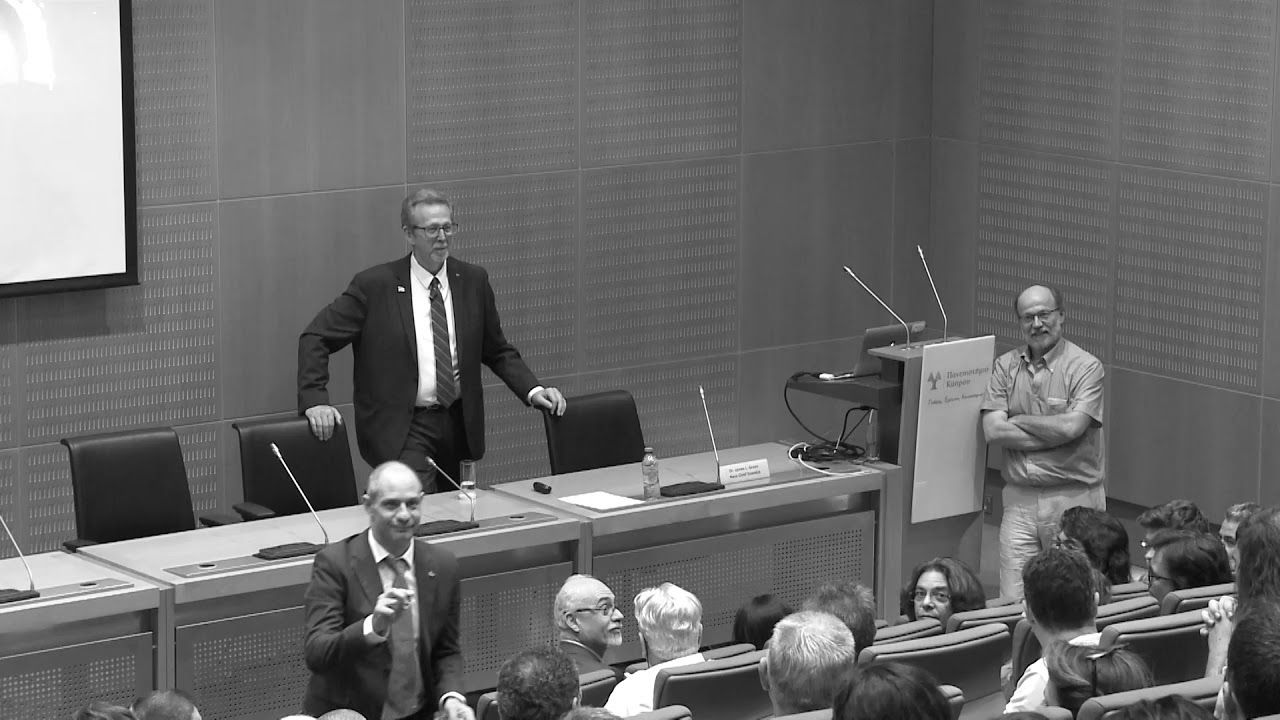
\includegraphics[width=1.0\textwidth]{./figures/nasa.jpg}
    %F.Ptochos hosting ``NASA Missions: From the Sun to Pluto and Beyond'' speech at University of Cyprus by Dr. James L. Green.
    
\vspace{0.3cm}
\large{Visit the favorite spots in town for amazing dishes and wine}
\begin{figure}
  \begin{center}
    %\vspace{6.5cm}
    \leavevmode
    \includegraphics[width=1.0\textwidth]{./figures/restaurants.png}
  \end{center}
\end{figure}
  
  \end{column}
\end{columns}

%\vspace{0.3cm}

\begin{columns}[T]
  \begin{column}{0.41\textwidth}
    %\begin{MyArticle}[enhanced, height=0.2\textheight,
%tikz={rotate=0}]{Physicists Find Elusive Particle Seen as Key to
%Universe}
\begin{MyArticle}[enhanced, tikz={rotate=0},
    width=1.0\textwidth]{\huge Physicists Find Elusive Particle Seen as Key to Universe}
  \begin{multicols}{2}
    Results are presented from searches for the standard model Higgs
    boson in proton–proton collisions at and 8 TeV in the Compact Muon
    Solenoid experiment at the LHC, using data samples corresponding
    to integrated luminosities of up to 5.1 fb$^{−1}$ at 7 TeV and 5.3 fb$^{−1}$
    at 8 TeV. The search is performed in five decay modes:
    $\gamma\gamma$, $ZZ$,  $\tau^{+}\tau^{-}$, and $b\bar{b}$.
    An excess of events is observed above the expected background,
    with a local significance of 5.0 standard deviations, at a mass
    near 125 GeV, signalling the production of a new particle. The
    expected significance for a standard model Higgs boson of that
    mass is 5.8 standard deviations. The excess is most significant in
    the two decay modes with the best mass resolution, $\gamma\gamma$ and $ZZ$; a
    fit to these signals gives a mass of 
    $125.3\pm0.4(\text{stat.})\pm0.5(\text{syst.})$ GeV. The decay to
    two photons indicates that the new particle is a boson with spin 
    different from one. 
    % ========================
    \begin{figure}
      \begin{center}
        \vspace{-0.2in}
        \leavevmode
        \includegraphics[width=0.5\textwidth]{./figures/HiggsBosonDiscoveryBW.png}
      \end{center}
    \end{figure}
    % ========================
  \end{multicols}
\end{MyArticle}

  \end{column}
  \begin{column}{0.01\textwidth}\end{column}
  \begin{column}{0.12\textwidth}
    \vspace{-0.5cm}
    \includegraphics[width=1.0\textwidth]{./figures/car.png}
    \vspace{0.5cm}
    \includegraphics[width=1.0\textwidth]{./figures/thkata.png}
    \vspace{0.2cm}
    
\includegraphics[width=1.0\textwidth]{./figures/Cyprus-in-your-heart.png}
  \end{column}
  \begin{column}{0.01\textwidth}\end{column}
  \begin{column}{0.4\textwidth}
    \begin{MyArticle}[enhanced, tikz={rotate=0},
  borderline={1mm}{0mm}{dotted}, width=1.0\textwidth]{Spooky Multi-Muon Events Puzzle Physicists}
  \begin{multicols}{2}
    CDF recently submitted a paper that helped to explain several long
    standing puzzles associated with the production of bottom quarks
    at the Tevatron. And in addition to solving these problems,
    researchers observed something perhaps even more interesting, a
    new, bigger puzzle.

    The work begins with a recent CDF measurement of the rate at which
    bottom and antibottom quarks are produced at the Tevatron. The
    analysis uses muons produced in the decay of bottom quarks to identify
    the signal events. Although previous measurements showed deviations
    from the predicted production rates, this newer, more precise
    measurement was found to agree well with the theoretical
    expectation. Interestingly, CDF found that the previous measurements
    could be explained by a source of background events that had not been
    previously identified. %Earlier analyses were unable to separate this
    %source of background from the bottom-quark signal, causing researchers
    %to miscount the number of bottom quarks produced.
    %

    % ========================
    \begin{figure}
      \begin{center}
      \leavevmode
      \includegraphics[width=0.45\textwidth]{./figures/Fotios-MinJeongKimBW.jpg}
      \end{center}
    \end{figure}
    % ========================
    
    The source of these background events, whimsically called \say{ghost
    events}, is the new puzzle. The properties of this background are
    quite different than background sources that had been previously
    identified. In particular, the ghost events contain more muons than
    are expected from known background sources.

    %The paper is just the beginning of the story. Ghost-busters have been
    %called in and are working to refine our understanding of these events
    %to see whether they provide evidence for new physics beyond the
    %Standard Model or whether these events exploited some lack of
    %understanding of the detector. The Tevatron may still have some
    %surprises in store for us, and only time will tell whether we should
    %believe in ghosts.
  \end{multicols}
    % ========================
    %\begin{figure}
    %  \begin{center}
    %    \vspace{-0.2in}
    %    \leavevmode
    %    \includegraphics[width=0.45\textwidth]{./figures/Fotios-MinJeongKimBW.jpg}
    %    %\caption*{The following physicists played a leading role in this analysis: From
    %    %  left to right: Min Jeong Kim, Fotis Ptohos, Fabio Happacher.}% Not shown: Paolo Giromini.}
    %  \end{center}
    %\end{figure}
    % ========================
  
\end{MyArticle}

  \end{column}  
  %\begin{column}{0.15\textwidth}
  %  \vspace{0.2cm}
  %  
\includegraphics[width=1.0\textwidth]{./figures/Cyprus-in-your-heart.png}
  %  \vspace{0.2cm}
  %  \includegraphics[width=1.0\textwidth]{./figures/thkata.png}
  %  \vspace{-0.5cm}
  %  \includegraphics[width=1.0\textwidth]{./figures/car.png}
  %\end{column}
  %\begin{column}{0.4\textwidth}
  %  \begin{MyArticle}[enhanced, tikz={rotate=0}, boxrule=1pt,
  titlerule=0pt, width=1.0\textwidth]{CDF publishes multi-muons!}
  \begin{multicols}{2}
    We report a study of multi-muon events produced at the
    Fermilab Tevatron collider and recorded by the CDF~II detector. In a data 
    set acquired with a dedicated dimuon trigger and corresponding to an 
    integrated luminosity of 2100 pb$^{-1}$, we isolate a significant sample of 
    events in which at least one of the muon candidates is produced 
    outside of the beam pipe of radius 1.5 cm. The production cross section
    and kinematics of events in which both muon candidates are produced inside
    the beam pipe are successfully modeled by known QCD processes which
    include heavy flavor production. In contrast, we are presently unable to 
    fully account for the number and properties of the remaining events, in which
    at least one muon candidate is produced outside of the beam pipe, in terms
    of the same understanding of the CDF~II detector, trigger, and event 
    reconstruction. Several topological and kinematic properties of these 
    events are presented in this paper. These events offer a plausible 
    resolution to long-standing inconsistencies related to $b\bar{b}$
    production and decay.
    \begin{comment}
    % ========================
    \begin{figure}
      \begin{center}
        \vspace{-0.2in}
        \leavevmode
        \includegraphics[width=\textwidth]{./figures/MultiMuons1BW_CDF.png}
        %\caption[] {Impact parameter distribution of muons contributed by ghost
        %  ($\bullet$) and QCD (histogram) events. Muon tracks are
        %  selected with loose SVX requirements. The detector resolution
        %  is $\simeq 30 \; \mu$m, whereas bins are 80 $\mu$m wide.} 
      \end{center}
    \end{figure}
    % ========================
    \end{comment}
  \end{multicols}
\end{MyArticle}

  %  \begin{multimuons-2}[enhanced, tikz={rotate=0}, width=1.0\textwidth]{Multi-Muons In CDF: The Mystery Continues}
  \begin{multicols}{2}
    We present a phenomenological conjecture of new physics that is suggested
    by the topology and kinematic properties of the multi-muon events recently
    reported by the CDF collaboration. We show that the salient features of 
    the data can be accounted for by postulating the pair production of
    three new states $h_1$, $h_2$, and $h_3$ with masses in the range
    of 15, 7.3, and 3.6 GeV/c$^{2}$, respectively. The heavier states 
    cascade-decay into the lighter ones, whereas the lightest state 
    decays into a $\tau$ pair with a lifetime of the order of 20 ps.
    \begin{comment}
    % ========================
    \begin{figure}
      \begin{center}
        \vspace{-0.2in}
        \leavevmode
        \includegraphics[width=\textwidth]{./figures/MultiMuons2_CDF.pdf}
        %\caption[]{Two-dimensional distributions, reproduced from Ref.~\cite{a0disc},
        %  of (a) the invariant mass, $M$, of all muons and (b) the total
        %  number of tracks contained in a $36.8^{\deg}$ cone when both
        %  cones contain at least two muons.}
      \end{center}
    \end{figure}
    % ========================
    \end{comment}
  \end{multicols}
\end{multimuons-2}

  %\end{column}
\end{columns}  

\vspace{-0.5cm}
\begin{columns}[T]
  \begin{column}{0.21\textwidth}
    \begin{MyArticle}[enhanced, tikz={rotate=0}, boxrule=1pt,
  titlerule=0pt, width=1.0\textwidth]{CDF publishes multi-muons!}
  \begin{multicols}{2}
    We report a study of multi-muon events produced at the
    Fermilab Tevatron collider and recorded by the CDF~II detector. In a data 
    set acquired with a dedicated dimuon trigger and corresponding to an 
    integrated luminosity of 2100 pb$^{-1}$, we isolate a significant sample of 
    events in which at least one of the muon candidates is produced 
    outside of the beam pipe of radius 1.5 cm. The production cross section
    and kinematics of events in which both muon candidates are produced inside
    the beam pipe are successfully modeled by known QCD processes which
    include heavy flavor production. In contrast, we are presently unable to 
    fully account for the number and properties of the remaining events, in which
    at least one muon candidate is produced outside of the beam pipe, in terms
    of the same understanding of the CDF~II detector, trigger, and event 
    reconstruction. Several topological and kinematic properties of these 
    events are presented in this paper. These events offer a plausible 
    resolution to long-standing inconsistencies related to $b\bar{b}$
    production and decay.
    \begin{comment}
    % ========================
    \begin{figure}
      \begin{center}
        \vspace{-0.2in}
        \leavevmode
        \includegraphics[width=\textwidth]{./figures/MultiMuons1BW_CDF.png}
        %\caption[] {Impact parameter distribution of muons contributed by ghost
        %  ($\bullet$) and QCD (histogram) events. Muon tracks are
        %  selected with loose SVX requirements. The detector resolution
        %  is $\simeq 30 \; \mu$m, whereas bins are 80 $\mu$m wide.} 
      \end{center}
    \end{figure}
    % ========================
    \end{comment}
  \end{multicols}
\end{MyArticle}

    %
\includegraphics[width=1.0\textwidth]{./figures/Nespresso4.jpg}
  \end{column}
  \begin{column}{0.36\textwidth}
    \begin{MyArticle}[enhanced, tikz={rotate=0}, width=0.3\textwidth]{Master of Masterclasses}
  \begin{multicols}{2}
    Another particle physics masterclass was organized at the University of Cyprus
    by Professor Fotios Ptochos for the 8$^{th}$ year
    in a row. It took within the framework of the IPPOG effort,  with
    the aim of informing young students about the research being
    carried out at CERN and the wider field of Particle Physics.
    Department of Physics. The event you took place on Saturday 07 March
    2020 at the University of Cyprus Campus between 9:00 - 17:00. It 
    included lectures about the world of elementary particles,
    detection methods, and the technology developed starting with
    basic research in both this and related fields of physics. Students had a unique opportunity to
    analyze data from proton-proton collisions, as recorded by the CMS
    detector at CERN's LHC. They discussed their
    findings with students from other countries as well as scientists
    at CERN through a video conference.
    \vspace{-0.5cm}
    % ========================
    \begin{figure}
      \begin{center}
        \leavevmode
        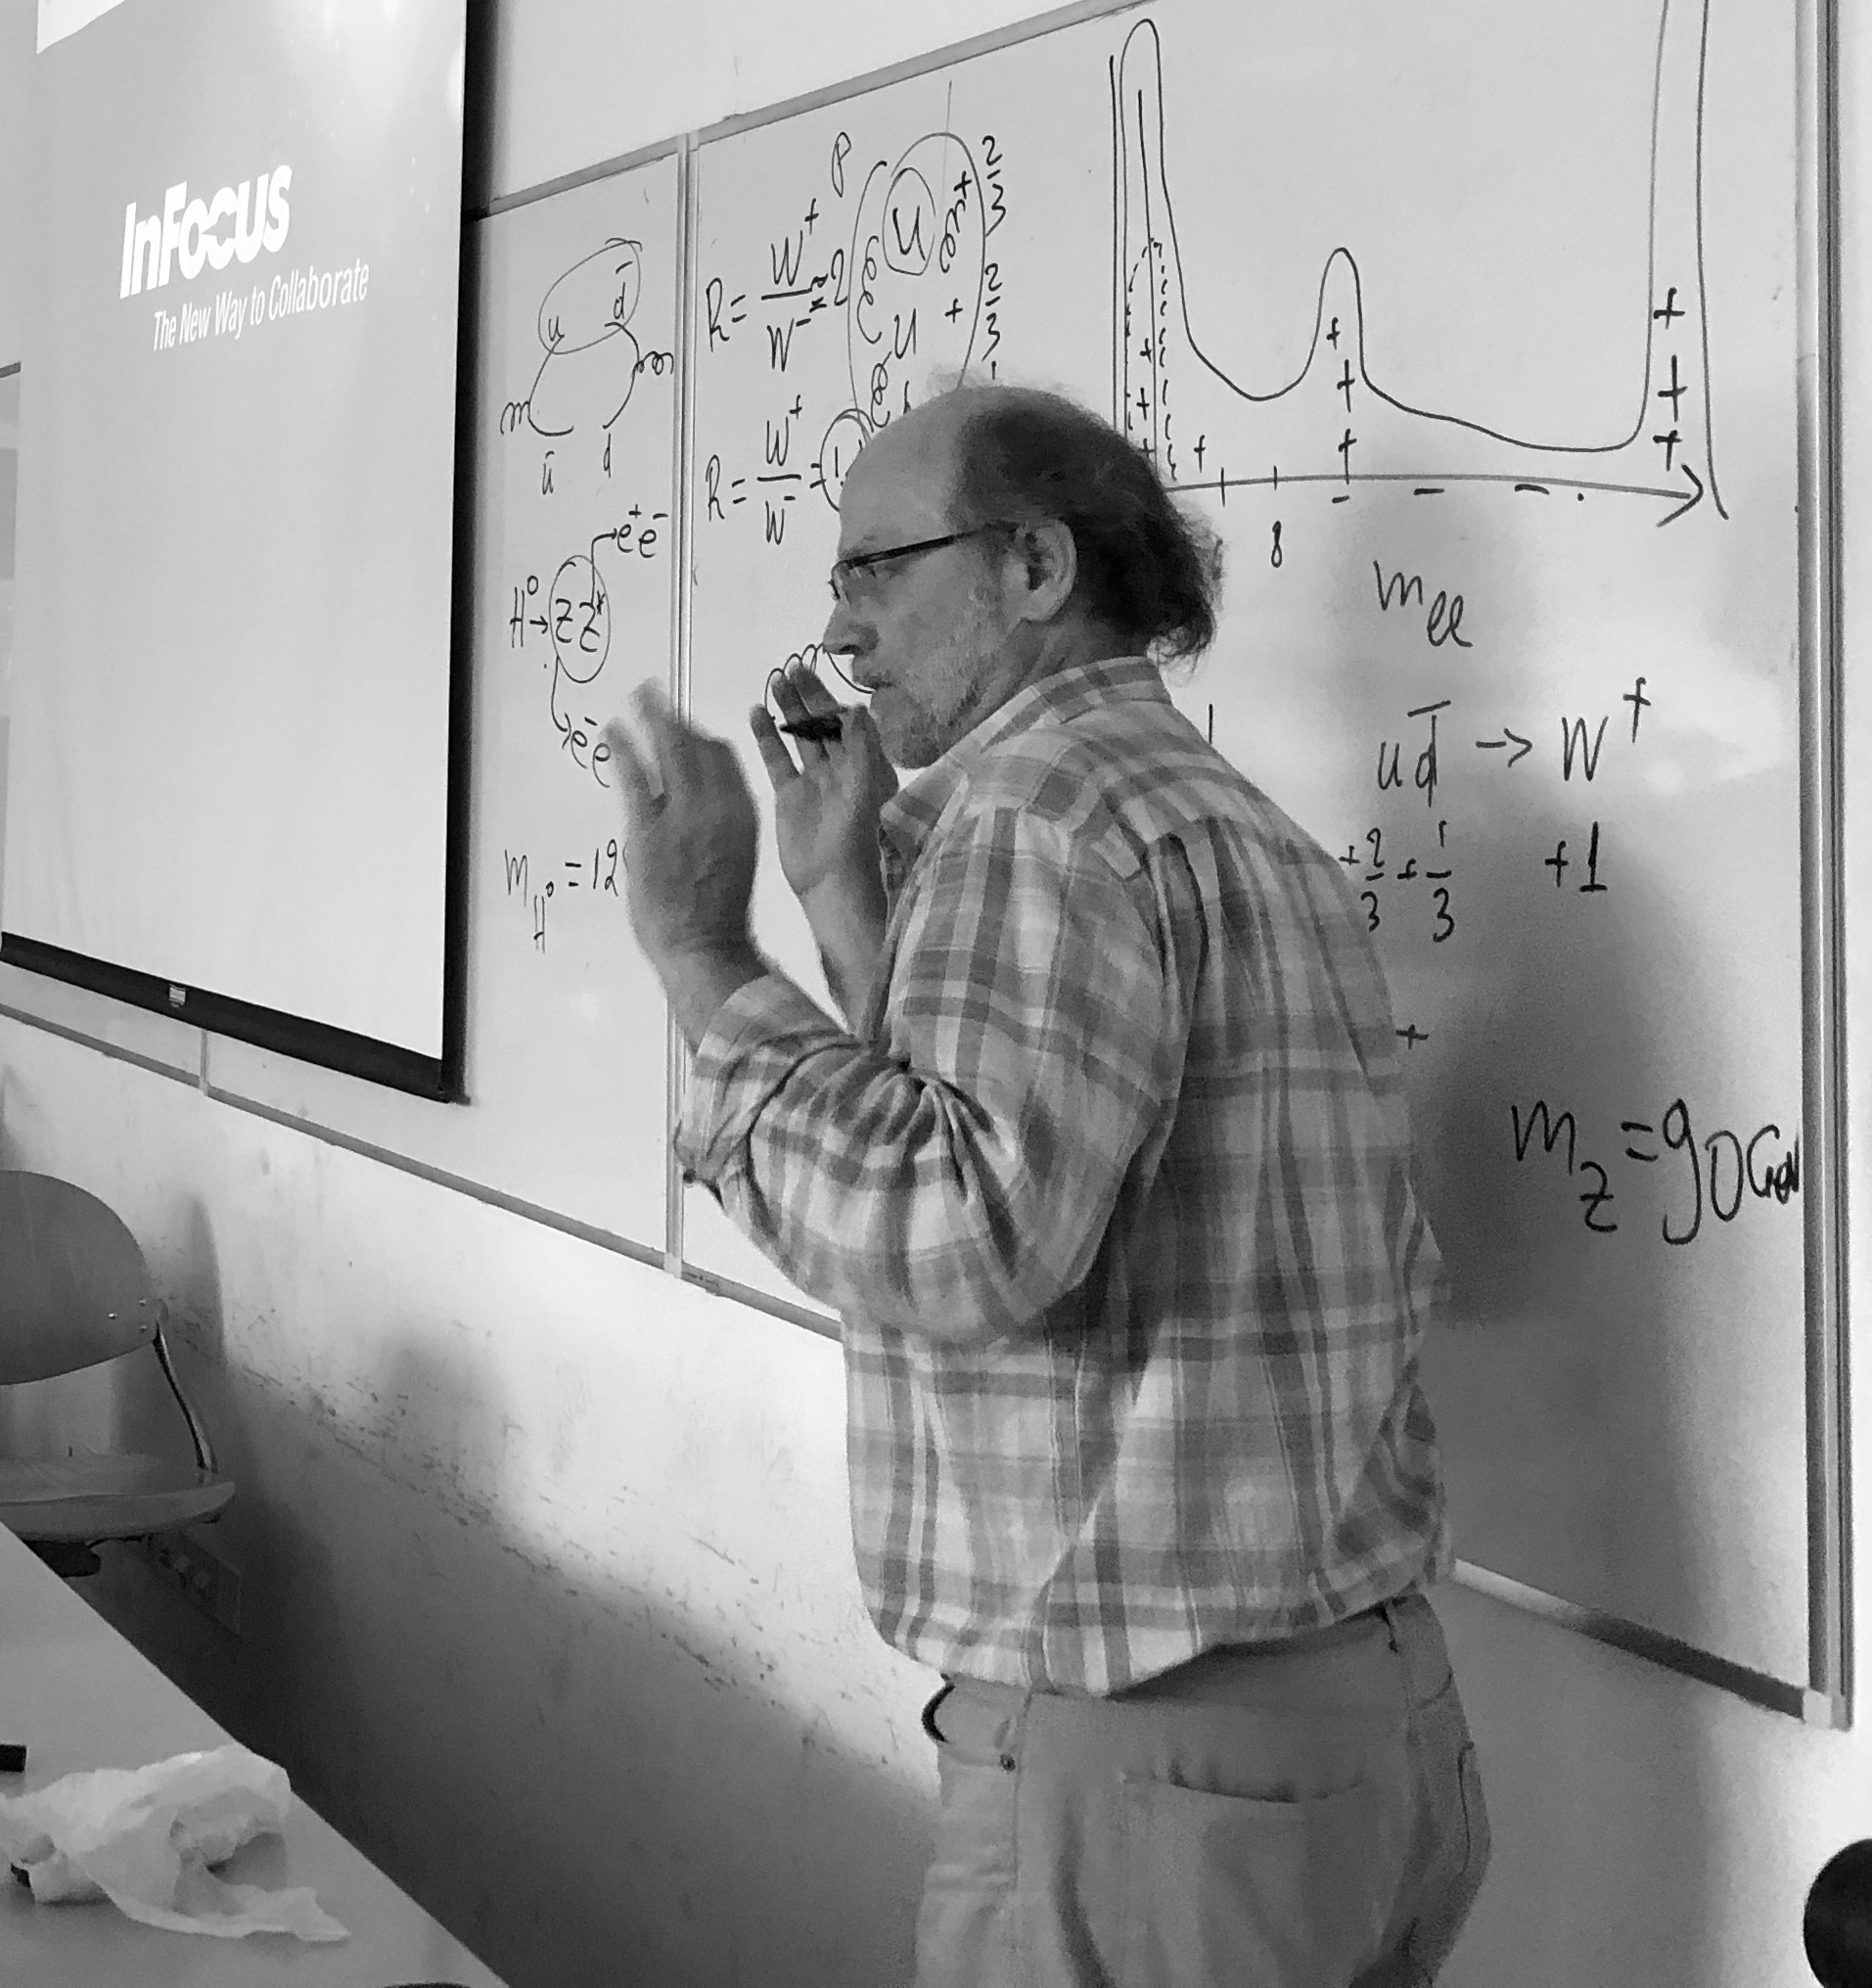
\includegraphics[width=0.45\textwidth]{./figures/Fotis6-narrow.png}
      \end{center}
    \end{figure}
    % ========================
  \end{multicols}
\end{MyArticle}

    \begin{multimuons-2}[enhanced, tikz={rotate=0}, width=1.0\textwidth]{Multi-Muons In CDF: The Mystery Continues}
  \begin{multicols}{2}
    We present a phenomenological conjecture of new physics that is suggested
    by the topology and kinematic properties of the multi-muon events recently
    reported by the CDF collaboration. We show that the salient features of 
    the data can be accounted for by postulating the pair production of
    three new states $h_1$, $h_2$, and $h_3$ with masses in the range
    of 15, 7.3, and 3.6 GeV/c$^{2}$, respectively. The heavier states 
    cascade-decay into the lighter ones, whereas the lightest state 
    decays into a $\tau$ pair with a lifetime of the order of 20 ps.
    \begin{comment}
    % ========================
    \begin{figure}
      \begin{center}
        \vspace{-0.2in}
        \leavevmode
        \includegraphics[width=\textwidth]{./figures/MultiMuons2_CDF.pdf}
        %\caption[]{Two-dimensional distributions, reproduced from Ref.~\cite{a0disc},
        %  of (a) the invariant mass, $M$, of all muons and (b) the total
        %  number of tracks contained in a $36.8^{\deg}$ cone when both
        %  cones contain at least two muons.}
      \end{center}
    \end{figure}
    % ========================
    \end{comment}
  \end{multicols}
\end{multimuons-2}

  \end{column}  
  \begin{column}{0.42\textwidth}
    \vspace{+0.3cm}
    \begin{MyArticleDotted}[enhanced, tikz={rotate=0}]{Search for charged Higgs bosons!} %
    A search for charged Higgs bosons ($H^{\pm}$) decaying into a top
    and a bottom quark in the all-jet final state is presented. The
    analysis uses LHC proton-proton collision data recorded with the
    CMS detector in 2016 at $\sqrt{s} = 13$ TeV, corresponding to an
    integrated luminosity of 35.9~$fb^{-1}$. No significant excess is
    observed above the expected background. Model-independent upper
    limits at 95$\%$ confidence level are set on the product of the
    $H^{\pm}$ production cross section and branching fraction in two
    scenarios.  For production in association with a top quark,
    limits of 21.3 to 0.007$pb$ are obtained for $H^{\pm}$ masses in the
    range of 0.2 to 3 TeV. Combining this with a search in leptonic
    final states results in improved limits of 9.25 to 0.005 $pb$. The
    complementary $s$-channel production of an $H^{\pm}$ is
    investigated in the mass range of 0.8 to 3 TeV and the
    corresponding upper limits are 4.5 to 0.023 $pb$. These results are
    interpreted using different minimal supersymmetric extensions of
    the standard model.
\end{MyArticleDotted}

    % Higgs boson: a tool to discover new physics: $H^{\pm}$
\begin{MyArticle}[enhanced, tikz={rotate=0}, boxrule=1pt, titlerule=0pt, width=1.0\textwidth]{New
    search for charged Higgs bosons in forgotten channels}
  \begin{multicols}{2}
  A search for a charged Higgs boson $H^{\pm}$ decaying
  into a heavy neutral Higgs boson $H$ and a $W$ boson
  is presented. The analysis targets the $W$ decay into a pair
  of tau leptons with at least one of them decaying hadronically and
  with an additional electron or muon present in the event.
  The search is based on proton-proton collision data
  recorded by the CMS experiment during 2016--2018 at
  $\sqrt{s} = 13~TeV$, corresponding to an integrated
  luminosity of 138~$fb^{-1}$. The data are consistent with
  standard model background expectations. Upper limits at 95$\%$ confidence
  level are set on the product of the cross section and branching fraction
  for an $H^{\pm}$ in the mass range of 300--700 GeV, assuming an $H$ 
  with a mass of 200 GeV. The observed limits range from
  0.085 $pb$ for an $H^{\pm}$ mass of
  300 $GeV$ to 0.019~$pb$ for a mass of
  700 $GeV$. These are the first limits on $H^{\pm}$
  production in the $H^{\pm} \to H W^{\pm}$ decay channel at the LHC. 
  \end{multicols}
\end{MyArticle}

  \end{column}
  %\begin{column}{0.33\textwidth}
  %  \begin{MyArticle}[enhanced, tikz={rotate=0}, width=1.0\textwidth]{From the Sun to Pluto and Beyond}
  \begin{multicols}{2}
  On \longdate\formatdate{19}{10}{2018} a public lecture was given by Dr. James L. Green, NASA Chief Scientist, at
  the University House \say{Anastasios G. Leventis} of the University
  of Cyprus with title ``NASA Missions: From the Sun to Pluto and Beyond''. The speaker was introduced by Associate Professor Fotios
  Ptochos, Chairperson of the Department of Physics. The event was
  organized by the University of Cyprus in cooperation with the
  U.S. Embassy Cyprus and Cyprus Space Exploration Organisation (CSEO).
  \vspace{-5mm}
  % ========================
  \begin{figure}
    \begin{center}
      \leavevmode
      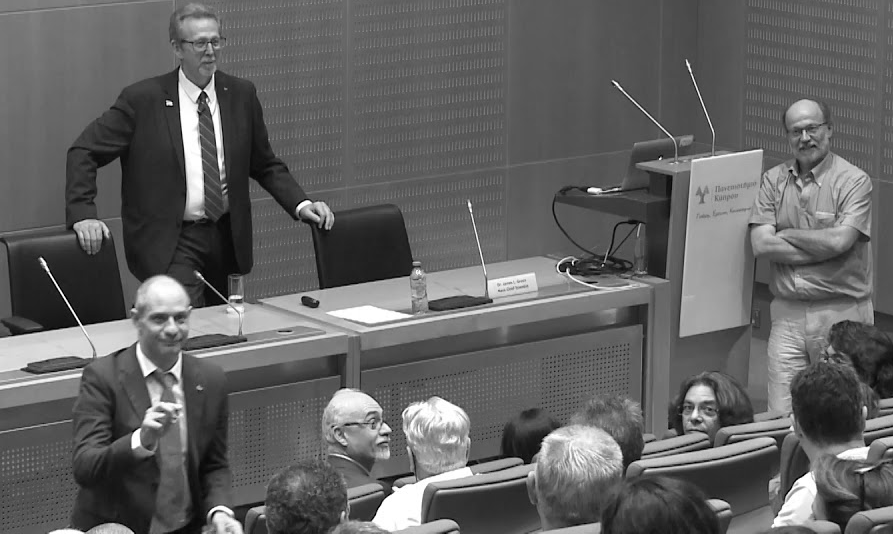
\includegraphics[width=0.5\textwidth]{./figures/NASA-small.png}
    \end{center}
  \end{figure}
  % ========================
  \end{multicols} 
\end{MyArticle}

  %\end{column}
\end{columns}

    %% CMS
%\begin{headline}[enhanced, tikz={rotate=0},
%width=1.0\textwidth]{Charged Higgs boson Hunting}
\begin{multimuons-1}[enhanced, tikz={rotate=0}, width=1.0\textwidth]{\huge Charged Higgs boson Hunting}

  \Large{$t\rightarrow bH^{\pm}\rightarrow \tau^{\pm} \nu_{\tau}$}............................\it{\Large 25 May 2012}\newline
  \Large{$H^{\pm}\rightarrow tb$ and $H^{\pm}\rightarrow \tau\nu$}..............\it{\Large 31 August 2015}\newline
  \Large{$H^{\pm} \rightarrow \tau^{\pm} \nu_{\tau}$}................................\it{\Large 11 March 2019}\newline
  \Large{$pp\rightarrow t(b)H^{\pm} \rightarrow tb$, all-jet}.......\it{\Large 21 January 2020}\newline
  \Large{$pp\rightarrow t(b)H^{\pm} \rightarrow W^{\pm}H^{0}(\tau\tau)$}...............\it{\Large 4 July 2022}
\end{multimuons-1}
 % https://cms-results.web.cern.ch/cms-results/public-results/publications/HIG-11-019/index.html
% https://cms-results.web.cern.ch/cms-results/public-results/publications/HIG-14-023/index.html
% https://cms-results.web.cern.ch/cms-results/public-results/publications/HIG-18-014/index.html
% https://cms-results.web.cern.ch/cms-results/public-results/publications/HIG-18-015/index.html
% https://cms-results.web.cern.ch/cms-results/public-results/publications/HIG-21-010/index.html

%    $t\rightarrow bH^{\pm}\rightarrow \tau^{\pm} \nu_{\tau}$.................\it{25 May 2012} \vspace{0.2cm} \newline
%    $H^{\pm}\rightarrow tb$ and $H^{\pm}\rightarrow \tau\nu$........\it{31 Aug 2015} \vspace{0.2cm} \newline
%    $H^{\pm} \rightarrow \tau^{\pm} \nu_{\tau}$ .........................\it{11 Mar 2019} \vspace{0.2cm} \newline
%    $pp\rightarrow t(b)H^{\pm} \rightarrow tb$, all-jet....\it{21 Jan 2020} \vspace{0.2cm} \newline
%    $pp\rightarrow t(b)H^{\pm} \rightarrow W^{\pm}H^{0}(\tau\tau)$......\it{4 Jul 2022}

    %\begin{tikzpicture}
%\node (Professor) at (current page.center) {%\begin{headline}[enhanced, tikz={rotate=0}]{Fotios Ptochos Promoted to Professor!}
\begin{headline}[enhanced, tikz={rotate=0}, width=1.0\textwidth]{Fotios Ptochos Promoted to Professor!}
\begin{multicols}{2}
    Congratulations to Fotios Ptochos for his promotion to the rank of
    Full Professor, effective from \MyDate. This promotion recognizes
    Prof. Ptochos' achievements in scholarship, teaching in physics
    and research in high-energy physics (HEP), and his overall service
    to the CDF and CMS Collaborations. He is a Harvard University PhD
    in physics graduate (1998) and has been active in HEP-research%,
    %both in detector development and physics analyses since 1987.
    since 1987. In particular, from 1987 to 1988 he worked in the development of
    a technique to monitor the purity of Liquid Argon (LAr) for the
    first ever prototype of the ICARUS detector.
    %, a technique that was subsequently used in the experiment. 
    From 1989 to 1994 he worked in the characterization of
    various Tetramethyl liquids as part of a research project to find
    appropriate warm liquids media for the envisioned calorimeter
    detectors at the Superconducting Supercollider (SSC).He also
    worked in the construction, installation and 
    calibration of the Central Muon Extension (CMX) system for the CDF
    detector. From 1994 to 1996 he developed an algorithm to improve
    electron identification for the CDF end-plug ECAL based on the
    information from the calorimeter and hits on the silicon tracker
    detector. The algorithm led to the development and implementation of
    the PHOENIX tracker system in the CDF-II detector. 
    %
    In the period of 2000–2003, he was the coordinator of the group
    responsible for the development, installation, maintenance and
    performance monitoring of the CDF-II Hadronic Calorimeter (HCAL)
    timing system. For the entire period of the Tevatron Run-II
    (2001-2011) he served as the coordinator of the CDF central HCAL
    calibration (CHA and WHA), maintenance and performance group. Since
    2004, when he joined the faculty of the UCY Physics Department, he has
    been involved in the UCY HEP group activities related to the
    construction and running of the CMS ECAL at CERN. In 2009, he
    initiated the involvement of the group in the activities related to
    the CMS tracking detector. He was also involved in the development of
    the dual-readout calorimetry concept in a total absorption HCAL for
    future linear-collider experiments. 
    % ========================
    \begin{figure}
      \begin{center}
      \leavevmode
      \includegraphics[width=0.45\textwidth]{./figures/Fotis7.png}
      \end{center}
    \end{figure}
    % ========================
    %
    % ========================
%    \begin{wrapfigure}{l}{0.33\textwidth}
%      \begin{center}
%        \includegraphics[width=0.22\textwidth]{./figures/Fotis7.png}
%      \end{center}
%      %\caption*{Fotios}
%    \end{wrapfigure}
    % ========================
    Professor Ptochos has led numerous physics analyses, spanning
    from precision measurements on properties of heavy flavour quark
    production and their use as probes for searching for the SM and SUSY
    Higgs bosons, to searches for BSM physics including SUSY, extra
    dimensions and other exotic processes. He has tremendous experience in
    heavy flavour tagging techniques and algorithms, tau-lepton
    identification techniques and new physics model building. 
    He was the first ever recipient of the \say{Fermi National
      Accelerator Laboratory Fellowship} and has co-coordinated multiple research program
    funded primarily by the European Commission (EC) via \textsc{Marie
    Skłodowska-Curie Actions},  the Cyprus Research Promotion
    Foundation (RPF) through \textsc{Didaktor} or \textsc{Excellence
      Hubs} programs, the European Regional Development Fund, and
    UCY. Professor Ptochos is the author and co-author of more than 
    1850 publications in refereed scientific journals and a member of the
    editorial group in charge for producing the education material
    for the entire Cyprus Secondary Education. He has been the
    supervisor of the research activities of 6 postdoctoral fellows, 5
    PhD and 11 MSc students, as well as projects of more than 20
    undergraduate students.  
\end{multicols}
\end{headline}

};  
%\node[left = 0.1cm of a] (b) {\begin{MyArticle}[enhanced, tikz={rotate=0}, boxrule=1pt,
  titlerule=0pt, width=1.0\textwidth]{CDF publishes multi-muons!}
  \begin{multicols}{2}
    We report a study of multi-muon events produced at the
    Fermilab Tevatron collider and recorded by the CDF~II detector. In a data 
    set acquired with a dedicated dimuon trigger and corresponding to an 
    integrated luminosity of 2100 pb$^{-1}$, we isolate a significant sample of 
    events in which at least one of the muon candidates is produced 
    outside of the beam pipe of radius 1.5 cm. The production cross section
    and kinematics of events in which both muon candidates are produced inside
    the beam pipe are successfully modeled by known QCD processes which
    include heavy flavor production. In contrast, we are presently unable to 
    fully account for the number and properties of the remaining events, in which
    at least one muon candidate is produced outside of the beam pipe, in terms
    of the same understanding of the CDF~II detector, trigger, and event 
    reconstruction. Several topological and kinematic properties of these 
    events are presented in this paper. These events offer a plausible 
    resolution to long-standing inconsistencies related to $b\bar{b}$
    production and decay.
    \begin{comment}
    % ========================
    \begin{figure}
      \begin{center}
        \vspace{-0.2in}
        \leavevmode
        \includegraphics[width=\textwidth]{./figures/MultiMuons1BW_CDF.png}
        %\caption[] {Impact parameter distribution of muons contributed by ghost
        %  ($\bullet$) and QCD (histogram) events. Muon tracks are
        %  selected with loose SVX requirements. The detector resolution
        %  is $\simeq 30 \; \mu$m, whereas bins are 80 $\mu$m wide.} 
      \end{center}
    \end{figure}
    % ========================
    \end{comment}
  \end{multicols}
\end{MyArticle}
};
%\node (Professor) at (0,0) {%\begin{headline}[enhanced, tikz={rotate=0}]{Fotios Ptochos Promoted to Professor!}
\begin{headline}[enhanced, tikz={rotate=0}, width=1.0\textwidth]{Fotios Ptochos Promoted to Professor!}
\begin{multicols}{2}
    Congratulations to Fotios Ptochos for his promotion to the rank of
    Full Professor, effective from \MyDate. This promotion recognizes
    Prof. Ptochos' achievements in scholarship, teaching in physics
    and research in high-energy physics (HEP), and his overall service
    to the CDF and CMS Collaborations. He is a Harvard University PhD
    in physics graduate (1998) and has been active in HEP-research%,
    %both in detector development and physics analyses since 1987.
    since 1987. In particular, from 1987 to 1988 he worked in the development of
    a technique to monitor the purity of Liquid Argon (LAr) for the
    first ever prototype of the ICARUS detector.
    %, a technique that was subsequently used in the experiment. 
    From 1989 to 1994 he worked in the characterization of
    various Tetramethyl liquids as part of a research project to find
    appropriate warm liquids media for the envisioned calorimeter
    detectors at the Superconducting Supercollider (SSC).He also
    worked in the construction, installation and 
    calibration of the Central Muon Extension (CMX) system for the CDF
    detector. From 1994 to 1996 he developed an algorithm to improve
    electron identification for the CDF end-plug ECAL based on the
    information from the calorimeter and hits on the silicon tracker
    detector. The algorithm led to the development and implementation of
    the PHOENIX tracker system in the CDF-II detector. 
    %
    In the period of 2000–2003, he was the coordinator of the group
    responsible for the development, installation, maintenance and
    performance monitoring of the CDF-II Hadronic Calorimeter (HCAL)
    timing system. For the entire period of the Tevatron Run-II
    (2001-2011) he served as the coordinator of the CDF central HCAL
    calibration (CHA and WHA), maintenance and performance group. Since
    2004, when he joined the faculty of the UCY Physics Department, he has
    been involved in the UCY HEP group activities related to the
    construction and running of the CMS ECAL at CERN. In 2009, he
    initiated the involvement of the group in the activities related to
    the CMS tracking detector. He was also involved in the development of
    the dual-readout calorimetry concept in a total absorption HCAL for
    future linear-collider experiments. 
    % ========================
    \begin{figure}
      \begin{center}
      \leavevmode
      \includegraphics[width=0.45\textwidth]{./figures/Fotis7.png}
      \end{center}
    \end{figure}
    % ========================
    %
    % ========================
%    \begin{wrapfigure}{l}{0.33\textwidth}
%      \begin{center}
%        \includegraphics[width=0.22\textwidth]{./figures/Fotis7.png}
%      \end{center}
%      %\caption*{Fotios}
%    \end{wrapfigure}
    % ========================
    Professor Ptochos has led numerous physics analyses, spanning
    from precision measurements on properties of heavy flavour quark
    production and their use as probes for searching for the SM and SUSY
    Higgs bosons, to searches for BSM physics including SUSY, extra
    dimensions and other exotic processes. He has tremendous experience in
    heavy flavour tagging techniques and algorithms, tau-lepton
    identification techniques and new physics model building. 
    He was the first ever recipient of the \say{Fermi National
      Accelerator Laboratory Fellowship} and has co-coordinated multiple research program
    funded primarily by the European Commission (EC) via \textsc{Marie
    Skłodowska-Curie Actions},  the Cyprus Research Promotion
    Foundation (RPF) through \textsc{Didaktor} or \textsc{Excellence
      Hubs} programs, the European Regional Development Fund, and
    UCY. Professor Ptochos is the author and co-author of more than 
    1850 publications in refereed scientific journals and a member of the
    editorial group in charge for producing the education material
    for the entire Cyprus Secondary Education. He has been the
    supervisor of the research activities of 6 postdoctoral fellows, 5
    PhD and 11 MSc students, as well as projects of more than 20
    undergraduate students.  
\end{multicols}
\end{headline}

};    
%\node[right = 0.2cm of Professor] (Higgs) {%\begin{MyArticle}[enhanced, height=0.2\textheight,
%tikz={rotate=0}]{Physicists Find Elusive Particle Seen as Key to
%Universe}
\begin{MyArticle}[enhanced, tikz={rotate=0},
    width=1.0\textwidth]{\huge Physicists Find Elusive Particle Seen as Key to Universe}
  \begin{multicols}{2}
    Results are presented from searches for the standard model Higgs
    boson in proton–proton collisions at and 8 TeV in the Compact Muon
    Solenoid experiment at the LHC, using data samples corresponding
    to integrated luminosities of up to 5.1 fb$^{−1}$ at 7 TeV and 5.3 fb$^{−1}$
    at 8 TeV. The search is performed in five decay modes:
    $\gamma\gamma$, $ZZ$,  $\tau^{+}\tau^{-}$, and $b\bar{b}$.
    An excess of events is observed above the expected background,
    with a local significance of 5.0 standard deviations, at a mass
    near 125 GeV, signalling the production of a new particle. The
    expected significance for a standard model Higgs boson of that
    mass is 5.8 standard deviations. The excess is most significant in
    the two decay modes with the best mass resolution, $\gamma\gamma$ and $ZZ$; a
    fit to these signals gives a mass of 
    $125.3\pm0.4(\text{stat.})\pm0.5(\text{syst.})$ GeV. The decay to
    two photons indicates that the new particle is a boson with spin 
    different from one. 
    % ========================
    \begin{figure}
      \begin{center}
        \vspace{-0.2in}
        \leavevmode
        \includegraphics[width=0.5\textwidth]{./figures/HiggsBosonDiscoveryBW.png}
      \end{center}
    \end{figure}
    % ========================
  \end{multicols}
\end{MyArticle}
};
%\node[above right = 0.2cm of Professor] (Multimuons2) {\begin{multimuons-2}[enhanced, tikz={rotate=0}, width=1.0\textwidth]{Multi-Muons In CDF: The Mystery Continues}
  \begin{multicols}{2}
    We present a phenomenological conjecture of new physics that is suggested
    by the topology and kinematic properties of the multi-muon events recently
    reported by the CDF collaboration. We show that the salient features of 
    the data can be accounted for by postulating the pair production of
    three new states $h_1$, $h_2$, and $h_3$ with masses in the range
    of 15, 7.3, and 3.6 GeV/c$^{2}$, respectively. The heavier states 
    cascade-decay into the lighter ones, whereas the lightest state 
    decays into a $\tau$ pair with a lifetime of the order of 20 ps.
    \begin{comment}
    % ========================
    \begin{figure}
      \begin{center}
        \vspace{-0.2in}
        \leavevmode
        \includegraphics[width=\textwidth]{./figures/MultiMuons2_CDF.pdf}
        %\caption[]{Two-dimensional distributions, reproduced from Ref.~\cite{a0disc},
        %  of (a) the invariant mass, $M$, of all muons and (b) the total
        %  number of tracks contained in a $36.8^{\deg}$ cone when both
        %  cones contain at least two muons.}
      \end{center}
    \end{figure}
    % ========================
    \end{comment}
  \end{multicols}
\end{multimuons-2}
};
%\node[left = 0.2cm of Multimuons2] (Multimuons1) {\begin{MyArticle}[enhanced, tikz={rotate=0}, boxrule=1pt,
  titlerule=0pt, width=1.0\textwidth]{CDF publishes multi-muons!}
  \begin{multicols}{2}
    We report a study of multi-muon events produced at the
    Fermilab Tevatron collider and recorded by the CDF~II detector. In a data 
    set acquired with a dedicated dimuon trigger and corresponding to an 
    integrated luminosity of 2100 pb$^{-1}$, we isolate a significant sample of 
    events in which at least one of the muon candidates is produced 
    outside of the beam pipe of radius 1.5 cm. The production cross section
    and kinematics of events in which both muon candidates are produced inside
    the beam pipe are successfully modeled by known QCD processes which
    include heavy flavor production. In contrast, we are presently unable to 
    fully account for the number and properties of the remaining events, in which
    at least one muon candidate is produced outside of the beam pipe, in terms
    of the same understanding of the CDF~II detector, trigger, and event 
    reconstruction. Several topological and kinematic properties of these 
    events are presented in this paper. These events offer a plausible 
    resolution to long-standing inconsistencies related to $b\bar{b}$
    production and decay.
    \begin{comment}
    % ========================
    \begin{figure}
      \begin{center}
        \vspace{-0.2in}
        \leavevmode
        \includegraphics[width=\textwidth]{./figures/MultiMuons1BW_CDF.png}
        %\caption[] {Impact parameter distribution of muons contributed by ghost
        %  ($\bullet$) and QCD (histogram) events. Muon tracks are
        %  selected with loose SVX requirements. The detector resolution
        %  is $\simeq 30 \; \mu$m, whereas bins are 80 $\mu$m wide.} 
      \end{center}
    \end{figure}
    % ========================
    \end{comment}
  \end{multicols}
\end{MyArticle}
};
%\node[left = 0.2cm of Multimuons1] (Higgs) {%\begin{MyArticle}[enhanced, height=0.2\textheight,
%tikz={rotate=0}]{Physicists Find Elusive Particle Seen as Key to
%Universe}
\begin{MyArticle}[enhanced, tikz={rotate=0},
    width=1.0\textwidth]{\huge Physicists Find Elusive Particle Seen as Key to Universe}
  \begin{multicols}{2}
    Results are presented from searches for the standard model Higgs
    boson in proton–proton collisions at and 8 TeV in the Compact Muon
    Solenoid experiment at the LHC, using data samples corresponding
    to integrated luminosities of up to 5.1 fb$^{−1}$ at 7 TeV and 5.3 fb$^{−1}$
    at 8 TeV. The search is performed in five decay modes:
    $\gamma\gamma$, $ZZ$,  $\tau^{+}\tau^{-}$, and $b\bar{b}$.
    An excess of events is observed above the expected background,
    with a local significance of 5.0 standard deviations, at a mass
    near 125 GeV, signalling the production of a new particle. The
    expected significance for a standard model Higgs boson of that
    mass is 5.8 standard deviations. The excess is most significant in
    the two decay modes with the best mass resolution, $\gamma\gamma$ and $ZZ$; a
    fit to these signals gives a mass of 
    $125.3\pm0.4(\text{stat.})\pm0.5(\text{syst.})$ GeV. The decay to
    two photons indicates that the new particle is a boson with spin 
    different from one. 
    % ========================
    \begin{figure}
      \begin{center}
        \vspace{-0.2in}
        \leavevmode
        \includegraphics[width=0.5\textwidth]{./figures/HiggsBosonDiscoveryBW.png}
      \end{center}
    \end{figure}
    % ========================
  \end{multicols}
\end{MyArticle}
};
%\end{tikzpicture}


%\tikz[overlay, remember picture] \node at (current page.center) {
%
%  \input{./tex/Professor_v4.tex}
%};

%\begin{multicols*}{2}
%  \input{./tex/Professor_v4.tex}
%  \columnbreak  
%  \begin{MyArticle}[enhanced, tikz={rotate=0}]{\huge Top Quark, Last Piece of Matter, Appears to Be in Place}
  \begin{multicols}{2}
    We establish the existence of the top quark using a 67 pb$^{-1}$ data
    sample of pp collisions at $\sqrt{s} = 1.8$ TeV collected with the Collider
    Detector at Fermilab (CDF). Employing techniques similar to those we
    previously published, we observe a signal consistent with $t\bar{t}$ decay to
    $WWbb$, but inconsistent with the background prediction by
    4.8$\sigma$. Additional evidence for the top quark is provided by a peak in
    the reconstructed mass distribution. We measure the top quark mass
    to be $176 \pm 8 (\text{stat.}) \pm 10 (\text{sys.})$ GeV/c$^{2}$,
    and the $t\bar{t}$ production cross section to be
    $6.8^{+3.6}_{-2.4}$ pb.
    % ========================
    \begin{figure}
      \begin{center}
        \vspace{-0.2in}
        \leavevmode
        %\includegraphics[width=0.5\textwidth]{./figures/TopQuark1.jpg}
        \includegraphics[width=0.5\textwidth]{./figures/TopQuark2BW.jpg}
      \end{center}
    \end{figure}
    % ========================
  \end{multicols}
\end{MyArticle}
  
%  
\vspace{0.3cm}
\large{Visit the favorite spots in town for amazing dishes and wine}
\begin{figure}
  \begin{center}
    %\vspace{6.5cm}
    \leavevmode
    \includegraphics[width=1.0\textwidth]{./figures/restaurants.png}
  \end{center}
\end{figure}

%  %\begin{MyArticle}[enhanced, height=0.2\textheight,
%tikz={rotate=0}]{Physicists Find Elusive Particle Seen as Key to
%Universe}
\begin{MyArticle}[enhanced, tikz={rotate=0},
    width=1.0\textwidth]{\huge Physicists Find Elusive Particle Seen as Key to Universe}
  \begin{multicols}{2}
    Results are presented from searches for the standard model Higgs
    boson in proton–proton collisions at and 8 TeV in the Compact Muon
    Solenoid experiment at the LHC, using data samples corresponding
    to integrated luminosities of up to 5.1 fb$^{−1}$ at 7 TeV and 5.3 fb$^{−1}$
    at 8 TeV. The search is performed in five decay modes:
    $\gamma\gamma$, $ZZ$,  $\tau^{+}\tau^{-}$, and $b\bar{b}$.
    An excess of events is observed above the expected background,
    with a local significance of 5.0 standard deviations, at a mass
    near 125 GeV, signalling the production of a new particle. The
    expected significance for a standard model Higgs boson of that
    mass is 5.8 standard deviations. The excess is most significant in
    the two decay modes with the best mass resolution, $\gamma\gamma$ and $ZZ$; a
    fit to these signals gives a mass of 
    $125.3\pm0.4(\text{stat.})\pm0.5(\text{syst.})$ GeV. The decay to
    two photons indicates that the new particle is a boson with spin 
    different from one. 
    % ========================
    \begin{figure}
      \begin{center}
        \vspace{-0.2in}
        \leavevmode
        \includegraphics[width=0.5\textwidth]{./figures/HiggsBosonDiscoveryBW.png}
      \end{center}
    \end{figure}
    % ========================
  \end{multicols}
\end{MyArticle}

%  %\begin{MyArticle}[enhanced, tikz={rotate=0}, boxrule=1pt,
  titlerule=0pt, width=1.0\textwidth]{CDF publishes multi-muons!}
  \begin{multicols}{2}
    We report a study of multi-muon events produced at the
    Fermilab Tevatron collider and recorded by the CDF~II detector. In a data 
    set acquired with a dedicated dimuon trigger and corresponding to an 
    integrated luminosity of 2100 pb$^{-1}$, we isolate a significant sample of 
    events in which at least one of the muon candidates is produced 
    outside of the beam pipe of radius 1.5 cm. The production cross section
    and kinematics of events in which both muon candidates are produced inside
    the beam pipe are successfully modeled by known QCD processes which
    include heavy flavor production. In contrast, we are presently unable to 
    fully account for the number and properties of the remaining events, in which
    at least one muon candidate is produced outside of the beam pipe, in terms
    of the same understanding of the CDF~II detector, trigger, and event 
    reconstruction. Several topological and kinematic properties of these 
    events are presented in this paper. These events offer a plausible 
    resolution to long-standing inconsistencies related to $b\bar{b}$
    production and decay.
    \begin{comment}
    % ========================
    \begin{figure}
      \begin{center}
        \vspace{-0.2in}
        \leavevmode
        \includegraphics[width=\textwidth]{./figures/MultiMuons1BW_CDF.png}
        %\caption[] {Impact parameter distribution of muons contributed by ghost
        %  ($\bullet$) and QCD (histogram) events. Muon tracks are
        %  selected with loose SVX requirements. The detector resolution
        %  is $\simeq 30 \; \mu$m, whereas bins are 80 $\mu$m wide.} 
      \end{center}
    \end{figure}
    % ========================
    \end{comment}
  \end{multicols}
\end{MyArticle}
 
%  %\input{./tex/CMS-HIG-18-015}
%  %% Higgs boson: a tool to discover new physics: $H^{\pm}$
\begin{MyArticle}[enhanced, tikz={rotate=0}, boxrule=1pt, titlerule=0pt, width=0.25\textwidth]{New
    search for charged Higgs bosons in forgotten channels}
  \begin{multicols}{2}
  A search for a charged Higgs boson $H^{\pm}$ decaying
  into a heavy neutral Higgs boson $H$ and a $W$ boson
  is presented. The analysis targets the $W$ decay into a pair
  of tau leptons with at least one of them decaying hadronically and
  with an additional electron or muon present in the event.
  The search is based on proton-proton collision data
  recorded by the CMS experiment during 2016--2018 at
  $\sqrt{s} = 13~TeV$, corresponding to an integrated
  luminosity of 138~$fb^{-1}$. The data are consistent with
  standard model background expectations. Upper limits at 95$\%$ confidence
  level are set on the product of the cross section and branching fraction
  for an $H^{\pm}$ in the mass range of 300--700 GeV, assuming an $H$ 
  with a mass of 200 GeV. The observed limits range from
  0.085 $pb$ for an $H^{\pm}$ mass of
  300 $GeV$ to 0.019~$pb$ for a mass of
  700 $GeV$. These are the first limits on $H^{\pm}$
  production in the $H^{\pm} \to H W^{\pm}$ decay channel at the LHC. 
  \end{multicols}
\end{MyArticle}

%\end{multicols*}
%\pagebreak
%
%  \begin{multicols*}{3}
%    %\input{./tex/FermilabToday.tex}  
%  
\vspace{0.3cm}
\large{Visit the favorite spots in town for amazing dishes and wine}
\begin{figure}
  \begin{center}
    %\vspace{6.5cm}
    \leavevmode
    \includegraphics[width=1.0\textwidth]{./figures/restaurants.png}
  \end{center}
\end{figure}

%    \columnbreak
%  
\vspace{0.3cm}
\large{Visit the favorite spots in town for amazing dishes and wine}
\begin{figure}
  \begin{center}
    %\vspace{6.5cm}
    \leavevmode
    \includegraphics[width=1.0\textwidth]{./figures/restaurants.png}
  \end{center}
\end{figure}

%  %\begin{MyArticle}[enhanced, tikz={rotate=0}]{\huge Top Quark, Last Piece of Matter, Appears to Be in Place}
  \begin{multicols}{2}
    We establish the existence of the top quark using a 67 pb$^{-1}$ data
    sample of pp collisions at $\sqrt{s} = 1.8$ TeV collected with the Collider
    Detector at Fermilab (CDF). Employing techniques similar to those we
    previously published, we observe a signal consistent with $t\bar{t}$ decay to
    $WWbb$, but inconsistent with the background prediction by
    4.8$\sigma$. Additional evidence for the top quark is provided by a peak in
    the reconstructed mass distribution. We measure the top quark mass
    to be $176 \pm 8 (\text{stat.}) \pm 10 (\text{sys.})$ GeV/c$^{2}$,
    and the $t\bar{t}$ production cross section to be
    $6.8^{+3.6}_{-2.4}$ pb.
    % ========================
    \begin{figure}
      \begin{center}
        \vspace{-0.2in}
        \leavevmode
        %\includegraphics[width=0.5\textwidth]{./figures/TopQuark1.jpg}
        \includegraphics[width=0.5\textwidth]{./figures/TopQuark2BW.jpg}
      \end{center}
    \end{figure}
    % ========================
  \end{multicols}
\end{MyArticle}
  
%  %\begin{MyArticle}[enhanced, tikz={rotate=0}, boxrule=1pt,
  titlerule=0pt, width=1.0\textwidth]{CDF publishes multi-muons!}
  \begin{multicols}{2}
    We report a study of multi-muon events produced at the
    Fermilab Tevatron collider and recorded by the CDF~II detector. In a data 
    set acquired with a dedicated dimuon trigger and corresponding to an 
    integrated luminosity of 2100 pb$^{-1}$, we isolate a significant sample of 
    events in which at least one of the muon candidates is produced 
    outside of the beam pipe of radius 1.5 cm. The production cross section
    and kinematics of events in which both muon candidates are produced inside
    the beam pipe are successfully modeled by known QCD processes which
    include heavy flavor production. In contrast, we are presently unable to 
    fully account for the number and properties of the remaining events, in which
    at least one muon candidate is produced outside of the beam pipe, in terms
    of the same understanding of the CDF~II detector, trigger, and event 
    reconstruction. Several topological and kinematic properties of these 
    events are presented in this paper. These events offer a plausible 
    resolution to long-standing inconsistencies related to $b\bar{b}$
    production and decay.
    \begin{comment}
    % ========================
    \begin{figure}
      \begin{center}
        \vspace{-0.2in}
        \leavevmode
        \includegraphics[width=\textwidth]{./figures/MultiMuons1BW_CDF.png}
        %\caption[] {Impact parameter distribution of muons contributed by ghost
        %  ($\bullet$) and QCD (histogram) events. Muon tracks are
        %  selected with loose SVX requirements. The detector resolution
        %  is $\simeq 30 \; \mu$m, whereas bins are 80 $\mu$m wide.} 
      \end{center}
    \end{figure}
    % ========================
    \end{comment}
  \end{multicols}
\end{MyArticle}

%  %
\vspace{0.3cm}
\large{Visit the favorite spots in town for amazing dishes and wine}
\begin{figure}
  \begin{center}
    %\vspace{6.5cm}
    \leavevmode
    \includegraphics[width=1.0\textwidth]{./figures/restaurants.png}
  \end{center}
\end{figure}
  
%  \begin{multimuons-2}[enhanced, tikz={rotate=0}, width=1.0\textwidth]{Multi-Muons In CDF: The Mystery Continues}
  \begin{multicols}{2}
    We present a phenomenological conjecture of new physics that is suggested
    by the topology and kinematic properties of the multi-muon events recently
    reported by the CDF collaboration. We show that the salient features of 
    the data can be accounted for by postulating the pair production of
    three new states $h_1$, $h_2$, and $h_3$ with masses in the range
    of 15, 7.3, and 3.6 GeV/c$^{2}$, respectively. The heavier states 
    cascade-decay into the lighter ones, whereas the lightest state 
    decays into a $\tau$ pair with a lifetime of the order of 20 ps.
    \begin{comment}
    % ========================
    \begin{figure}
      \begin{center}
        \vspace{-0.2in}
        \leavevmode
        \includegraphics[width=\textwidth]{./figures/MultiMuons2_CDF.pdf}
        %\caption[]{Two-dimensional distributions, reproduced from Ref.~\cite{a0disc},
        %  of (a) the invariant mass, $M$, of all muons and (b) the total
        %  number of tracks contained in a $36.8^{\deg}$ cone when both
        %  cones contain at least two muons.}
      \end{center}
    \end{figure}
    % ========================
    \end{comment}
  \end{multicols}
\end{multimuons-2}

%\end{multicols*}


%\input{./tex/AdsVarious.tex}
% \input{./tex/AdsRestaurant.tex}
% \input{./tex/CMS-HIG-18-015}
% % Higgs boson: a tool to discover new physics: $H^{\pm}$
\begin{MyArticle}[enhanced, tikz={rotate=0}, boxrule=1pt, titlerule=0pt, width=0.25\textwidth]{New
    search for charged Higgs bosons in forgotten channels}
  \begin{multicols}{2}
  A search for a charged Higgs boson $H^{\pm}$ decaying
  into a heavy neutral Higgs boson $H$ and a $W$ boson
  is presented. The analysis targets the $W$ decay into a pair
  of tau leptons with at least one of them decaying hadronically and
  with an additional electron or muon present in the event.
  The search is based on proton-proton collision data
  recorded by the CMS experiment during 2016--2018 at
  $\sqrt{s} = 13~TeV$, corresponding to an integrated
  luminosity of 138~$fb^{-1}$. The data are consistent with
  standard model background expectations. Upper limits at 95$\%$ confidence
  level are set on the product of the cross section and branching fraction
  for an $H^{\pm}$ in the mass range of 300--700 GeV, assuming an $H$ 
  with a mass of 200 GeV. The observed limits range from
  0.085 $pb$ for an $H^{\pm}$ mass of
  300 $GeV$ to 0.019~$pb$ for a mass of
  700 $GeV$. These are the first limits on $H^{\pm}$
  production in the $H^{\pm} \to H W^{\pm}$ decay channel at the LHC. 
  \end{multicols}
\end{MyArticle}

% \input{./tex/FermilabToday.tex}
% \input{./tex/HExtended.tex}
% %\begin{MyArticle}[enhanced, height=0.2\textheight,
%tikz={rotate=0}]{Physicists Find Elusive Particle Seen as Key to
%Universe}
\begin{MyArticle}[enhanced, tikz={rotate=0},
    width=1.0\textwidth]{\huge Physicists Find Elusive Particle Seen as Key to Universe}
  \begin{multicols}{2}
    Results are presented from searches for the standard model Higgs
    boson in proton–proton collisions at and 8 TeV in the Compact Muon
    Solenoid experiment at the LHC, using data samples corresponding
    to integrated luminosities of up to 5.1 fb$^{−1}$ at 7 TeV and 5.3 fb$^{−1}$
    at 8 TeV. The search is performed in five decay modes:
    $\gamma\gamma$, $ZZ$,  $\tau^{+}\tau^{-}$, and $b\bar{b}$.
    An excess of events is observed above the expected background,
    with a local significance of 5.0 standard deviations, at a mass
    near 125 GeV, signalling the production of a new particle. The
    expected significance for a standard model Higgs boson of that
    mass is 5.8 standard deviations. The excess is most significant in
    the two decay modes with the best mass resolution, $\gamma\gamma$ and $ZZ$; a
    fit to these signals gives a mass of 
    $125.3\pm0.4(\text{stat.})\pm0.5(\text{syst.})$ GeV. The decay to
    two photons indicates that the new particle is a boson with spin 
    different from one. 
    % ========================
    \begin{figure}
      \begin{center}
        \vspace{-0.2in}
        \leavevmode
        \includegraphics[width=0.5\textwidth]{./figures/HiggsBosonDiscoveryBW.png}
      \end{center}
    \end{figure}
    % ========================
  \end{multicols}
\end{MyArticle}

% \begin{MyArticle}[enhanced, tikz={rotate=0}, boxrule=1pt,
  titlerule=0pt, width=1.0\textwidth]{CDF publishes multi-muons!}
  \begin{multicols}{2}
    We report a study of multi-muon events produced at the
    Fermilab Tevatron collider and recorded by the CDF~II detector. In a data 
    set acquired with a dedicated dimuon trigger and corresponding to an 
    integrated luminosity of 2100 pb$^{-1}$, we isolate a significant sample of 
    events in which at least one of the muon candidates is produced 
    outside of the beam pipe of radius 1.5 cm. The production cross section
    and kinematics of events in which both muon candidates are produced inside
    the beam pipe are successfully modeled by known QCD processes which
    include heavy flavor production. In contrast, we are presently unable to 
    fully account for the number and properties of the remaining events, in which
    at least one muon candidate is produced outside of the beam pipe, in terms
    of the same understanding of the CDF~II detector, trigger, and event 
    reconstruction. Several topological and kinematic properties of these 
    events are presented in this paper. These events offer a plausible 
    resolution to long-standing inconsistencies related to $b\bar{b}$
    production and decay.
    \begin{comment}
    % ========================
    \begin{figure}
      \begin{center}
        \vspace{-0.2in}
        \leavevmode
        \includegraphics[width=\textwidth]{./figures/MultiMuons1BW_CDF.png}
        %\caption[] {Impact parameter distribution of muons contributed by ghost
        %  ($\bullet$) and QCD (histogram) events. Muon tracks are
        %  selected with loose SVX requirements. The detector resolution
        %  is $\simeq 30 \; \mu$m, whereas bins are 80 $\mu$m wide.} 
      \end{center}
    \end{figure}
    % ========================
    \end{comment}
  \end{multicols}
\end{MyArticle}
 
% \begin{multimuons-2}[enhanced, tikz={rotate=0}, width=1.0\textwidth]{Multi-Muons In CDF: The Mystery Continues}
  \begin{multicols}{2}
    We present a phenomenological conjecture of new physics that is suggested
    by the topology and kinematic properties of the multi-muon events recently
    reported by the CDF collaboration. We show that the salient features of 
    the data can be accounted for by postulating the pair production of
    three new states $h_1$, $h_2$, and $h_3$ with masses in the range
    of 15, 7.3, and 3.6 GeV/c$^{2}$, respectively. The heavier states 
    cascade-decay into the lighter ones, whereas the lightest state 
    decays into a $\tau$ pair with a lifetime of the order of 20 ps.
    \begin{comment}
    % ========================
    \begin{figure}
      \begin{center}
        \vspace{-0.2in}
        \leavevmode
        \includegraphics[width=\textwidth]{./figures/MultiMuons2_CDF.pdf}
        %\caption[]{Two-dimensional distributions, reproduced from Ref.~\cite{a0disc},
        %  of (a) the invariant mass, $M$, of all muons and (b) the total
        %  number of tracks contained in a $36.8^{\deg}$ cone when both
        %  cones contain at least two muons.}
      \end{center}
    \end{figure}
    % ========================
    \end{comment}
  \end{multicols}
\end{multimuons-2}
  
% \begin{MyArticle}[enhanced, tikz={rotate=0}]{\huge Top Quark, Last Piece of Matter, Appears to Be in Place}
  \begin{multicols}{2}
    We establish the existence of the top quark using a 67 pb$^{-1}$ data
    sample of pp collisions at $\sqrt{s} = 1.8$ TeV collected with the Collider
    Detector at Fermilab (CDF). Employing techniques similar to those we
    previously published, we observe a signal consistent with $t\bar{t}$ decay to
    $WWbb$, but inconsistent with the background prediction by
    4.8$\sigma$. Additional evidence for the top quark is provided by a peak in
    the reconstructed mass distribution. We measure the top quark mass
    to be $176 \pm 8 (\text{stat.}) \pm 10 (\text{sys.})$ GeV/c$^{2}$,
    and the $t\bar{t}$ production cross section to be
    $6.8^{+3.6}_{-2.4}$ pb.
    % ========================
    \begin{figure}
      \begin{center}
        \vspace{-0.2in}
        \leavevmode
        %\includegraphics[width=0.5\textwidth]{./figures/TopQuark1.jpg}
        \includegraphics[width=0.5\textwidth]{./figures/TopQuark2BW.jpg}
      \end{center}
    \end{figure}
    % ========================
  \end{multicols}
\end{MyArticle}

% \input{./tex/ads.tex}


%   \begin{multicols*}{3}
%    \begin{MyArticle}[enhanced, tikz={rotate=0}, boxrule=1pt,
  titlerule=0pt, width=1.0\textwidth]{CDF publishes multi-muons!}
  \begin{multicols}{2}
    We report a study of multi-muon events produced at the
    Fermilab Tevatron collider and recorded by the CDF~II detector. In a data 
    set acquired with a dedicated dimuon trigger and corresponding to an 
    integrated luminosity of 2100 pb$^{-1}$, we isolate a significant sample of 
    events in which at least one of the muon candidates is produced 
    outside of the beam pipe of radius 1.5 cm. The production cross section
    and kinematics of events in which both muon candidates are produced inside
    the beam pipe are successfully modeled by known QCD processes which
    include heavy flavor production. In contrast, we are presently unable to 
    fully account for the number and properties of the remaining events, in which
    at least one muon candidate is produced outside of the beam pipe, in terms
    of the same understanding of the CDF~II detector, trigger, and event 
    reconstruction. Several topological and kinematic properties of these 
    events are presented in this paper. These events offer a plausible 
    resolution to long-standing inconsistencies related to $b\bar{b}$
    production and decay.
    \begin{comment}
    % ========================
    \begin{figure}
      \begin{center}
        \vspace{-0.2in}
        \leavevmode
        \includegraphics[width=\textwidth]{./figures/MultiMuons1BW_CDF.png}
        %\caption[] {Impact parameter distribution of muons contributed by ghost
        %  ($\bullet$) and QCD (histogram) events. Muon tracks are
        %  selected with loose SVX requirements. The detector resolution
        %  is $\simeq 30 \; \mu$m, whereas bins are 80 $\mu$m wide.} 
      \end{center}
    \end{figure}
    % ========================
    \end{comment}
  \end{multicols}
\end{MyArticle}

%    \columnbreak
%    \input{./tex/Professor_v4.tex}
%    \columnbreak
%    \begin{multimuons-2}[enhanced, tikz={rotate=0}, width=1.0\textwidth]{Multi-Muons In CDF: The Mystery Continues}
  \begin{multicols}{2}
    We present a phenomenological conjecture of new physics that is suggested
    by the topology and kinematic properties of the multi-muon events recently
    reported by the CDF collaboration. We show that the salient features of 
    the data can be accounted for by postulating the pair production of
    three new states $h_1$, $h_2$, and $h_3$ with masses in the range
    of 15, 7.3, and 3.6 GeV/c$^{2}$, respectively. The heavier states 
    cascade-decay into the lighter ones, whereas the lightest state 
    decays into a $\tau$ pair with a lifetime of the order of 20 ps.
    \begin{comment}
    % ========================
    \begin{figure}
      \begin{center}
        \vspace{-0.2in}
        \leavevmode
        \includegraphics[width=\textwidth]{./figures/MultiMuons2_CDF.pdf}
        %\caption[]{Two-dimensional distributions, reproduced from Ref.~\cite{a0disc},
        %  of (a) the invariant mass, $M$, of all muons and (b) the total
        %  number of tracks contained in a $36.8^{\deg}$ cone when both
        %  cones contain at least two muons.}
      \end{center}
    \end{figure}
    % ========================
    \end{comment}
  \end{multicols}
\end{multimuons-2}
  
%  %   \vfill
%  %   \input{./tex/CMS-HIG-18-015}
%  %   
%  %   \columnbreak
%  %   \begin{MyArticle}[enhanced, tikz={rotate=0}]{\huge Top Quark, Last Piece of Matter, Appears to Be in Place}
  \begin{multicols}{2}
    We establish the existence of the top quark using a 67 pb$^{-1}$ data
    sample of pp collisions at $\sqrt{s} = 1.8$ TeV collected with the Collider
    Detector at Fermilab (CDF). Employing techniques similar to those we
    previously published, we observe a signal consistent with $t\bar{t}$ decay to
    $WWbb$, but inconsistent with the background prediction by
    4.8$\sigma$. Additional evidence for the top quark is provided by a peak in
    the reconstructed mass distribution. We measure the top quark mass
    to be $176 \pm 8 (\text{stat.}) \pm 10 (\text{sys.})$ GeV/c$^{2}$,
    and the $t\bar{t}$ production cross section to be
    $6.8^{+3.6}_{-2.4}$ pb.
    % ========================
    \begin{figure}
      \begin{center}
        \vspace{-0.2in}
        \leavevmode
        %\includegraphics[width=0.5\textwidth]{./figures/TopQuark1.jpg}
        \includegraphics[width=0.5\textwidth]{./figures/TopQuark2BW.jpg}
      \end{center}
    \end{figure}
    % ========================
  \end{multicols}
\end{MyArticle}

%  
%   \end{multicols*}
    


\end{document}

